\documentclass[10pt]{article}
\usepackage[margin=2.0cm]{geometry}
\usepackage{graphicx}\usepackage{booktabs}\usepackage{amsmath}\usepackage{amssymb}
\usepackage{xcolor}\usepackage[hidelinks]{hyperref}
\setlength{\parskip}{4pt}\setlength{\parindent}{0pt}
\graphicspath{{../../../output/06_monte_carlo/}{../../../output/00_overview/}}
\title{\vspace{-1.2cm}\textbf{Review 06 --- Monte-Carlo focal field (clear limit + initialization proof)}\\
\large \texttt{mcdo\_dev} Phase 6a \quad(\texttt{output/06\_monte\_carlo/},
\texttt{docs/theory/06\_monte\_carlo.md})}
\author{}\date{2026-06-14}
\begin{document}\maketitle\vspace{-1.0cm}

\section*{0. Where this sits --- the pipeline}
Every model since Romallosa runs the same pipeline: a pupil $A(\theta)$
(+ polarization, + spectrum) is focused by an aplanatic system --- the
Debye--Wolf integral \emph{or} its Monte-Carlo plane-wave equivalent --- into a
focal field, then scored by FWHM / zeros / Linfoot / DOF / Strehl. The MC
\emph{clear limit equals} the Debye--Wolf integral; that equality is the
validation gate this review establishes.
\begin{center}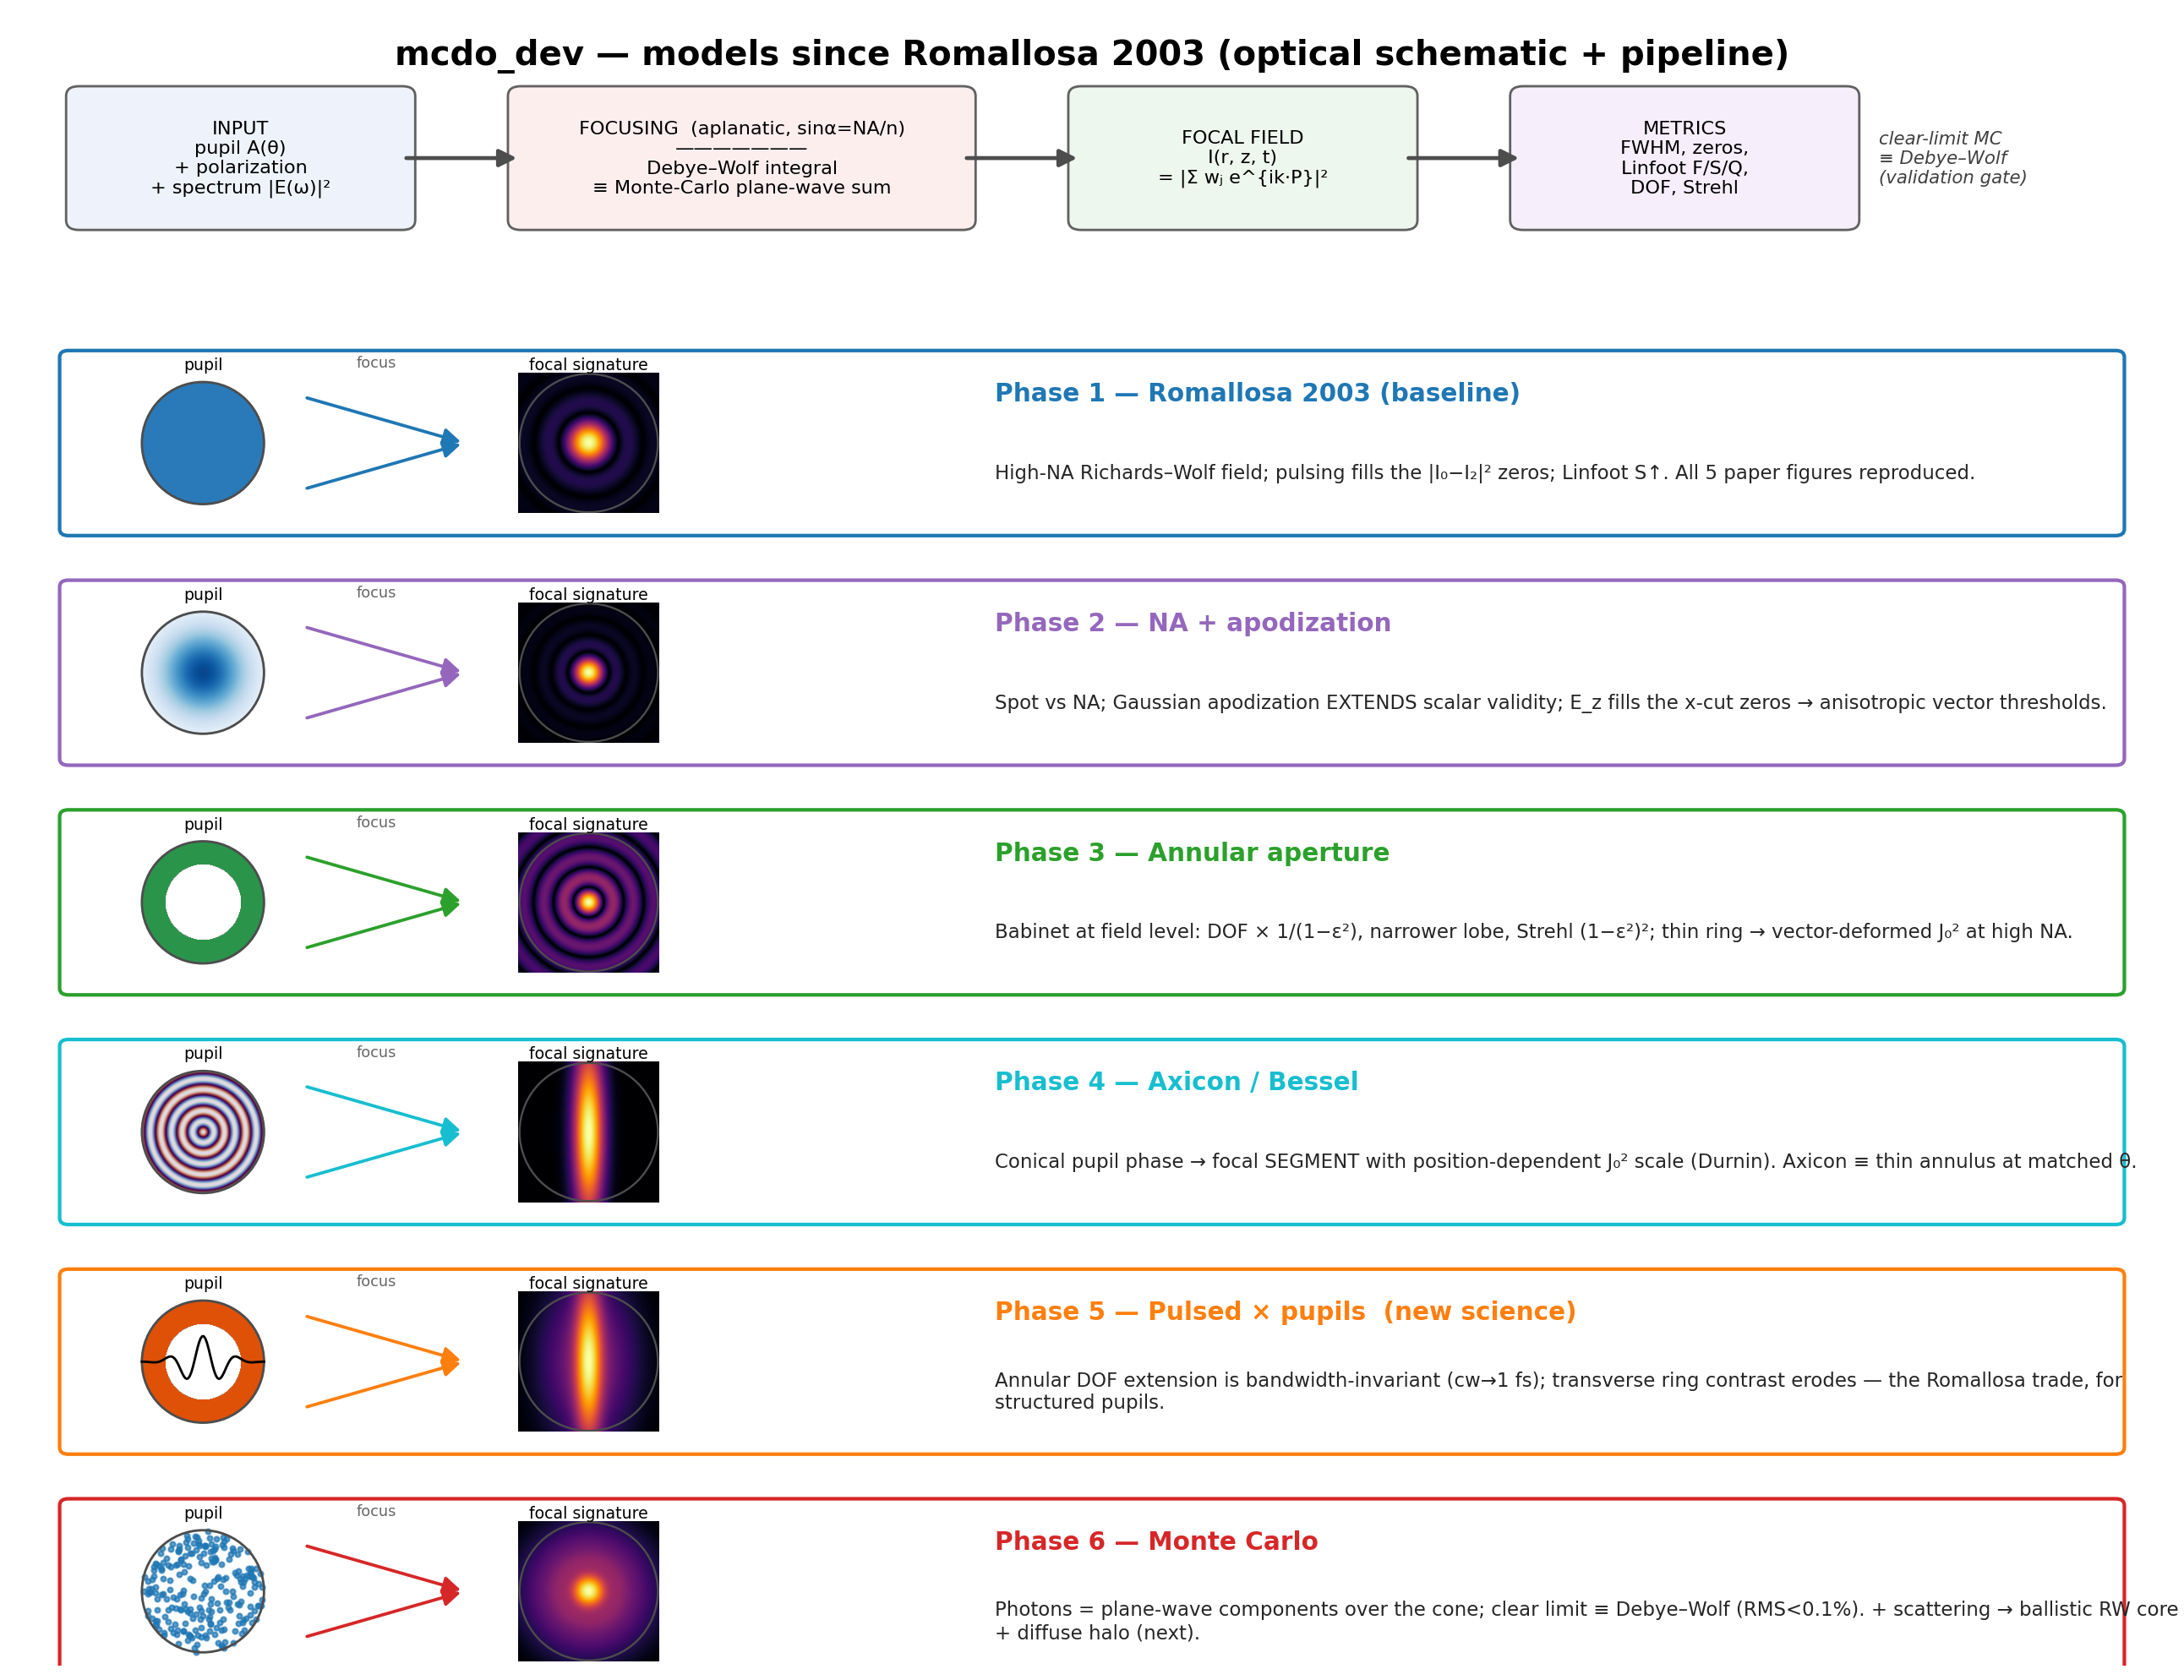
\includegraphics[width=0.97\textwidth]{models_schematic.png}\end{center}

\section*{1. Why a photon is a plane wave, and the clear-limit gate}
A photon is a plane-wave (angular-spectrum) component of the converging field,
$U(P)=\sum_j w_j\,e^{ik\hat{k}_j\cdot P}$. With $\mu_s=0$ this is a Monte-Carlo
evaluation of the Debye--Wolf integral, so it must converge to Richards--Wolf
($X_{NA}=0.8$, scalar):
\begin{center}\small\begin{tabular}{lcc}\toprule
$N$ & RMS vs deterministic & null floor\\\midrule
$10^3$ & 0.0117 & $4.4\times10^{-3}$\\
$10^4$ & 0.0033 & $5.3\times10^{-4}$\\
$10^5$ & 0.0008 & $\sim5\times10^{-4}$\\\bottomrule
\end{tabular}\end{center}
Null floor $\propto 1/N$ (random-walk residual at the true zeros); low-NA matches
the analytic Airy to 0.0015.
\begin{center}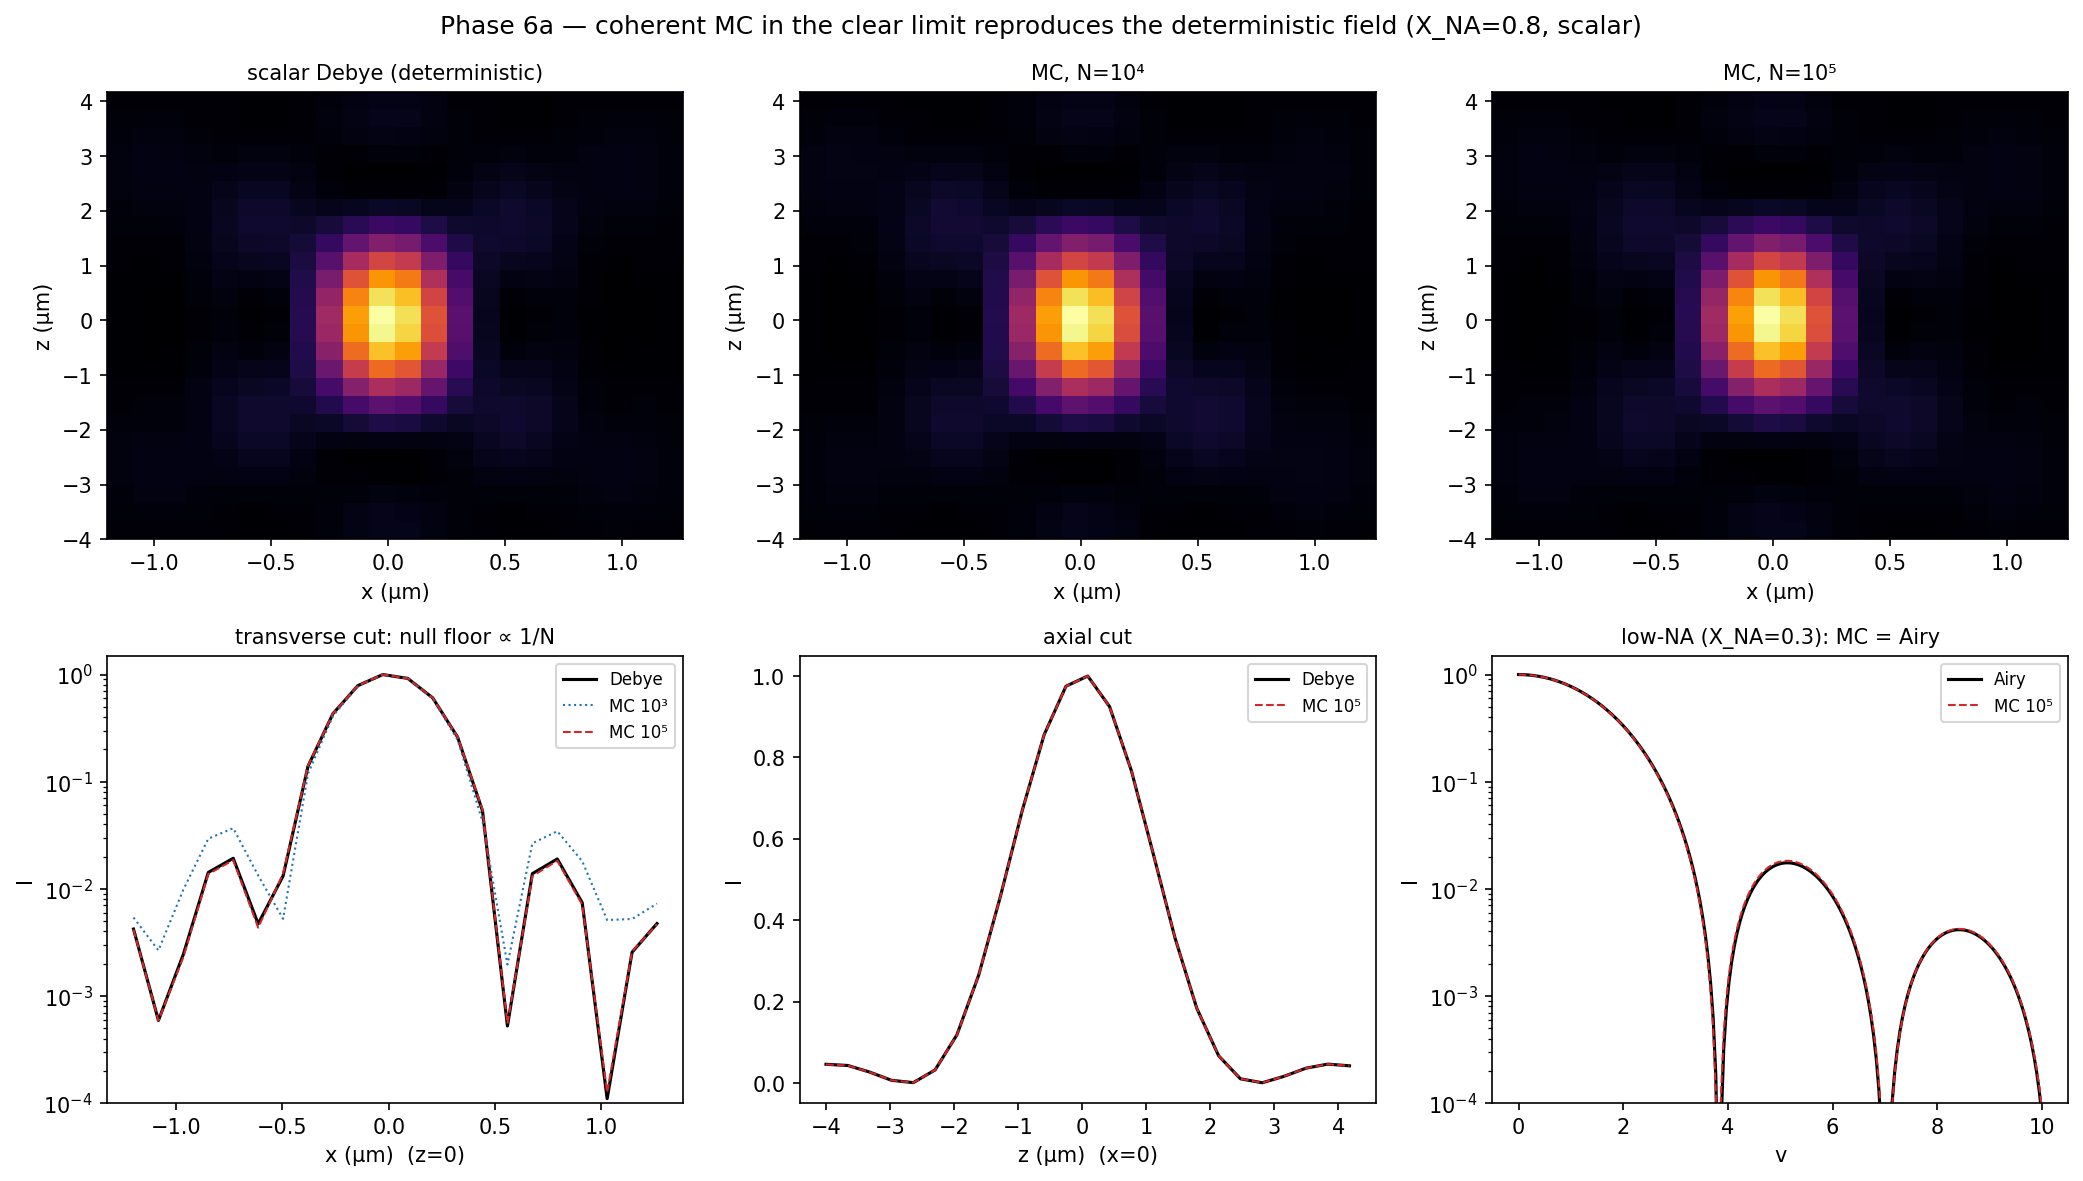
\includegraphics[width=0.9\textwidth]{verify_mc_clear.png}\end{center}

\section*{2. Per-configuration proof}
Same scalar Debye integral, deterministic vs MC photons ($N=10^5$, RMS over the
$x$--$z$ slice):
\begin{center}\small\begin{tabular}{lc}\toprule
configuration & RMS\\\midrule
uniform & 0.0006\\ Gaussian $\alpha_t=2$ & 0.0010\\
annular $\varepsilon=0.5$ & 0.0009\\ axicon $\beta=20$ & 0.0018\\\bottomrule
\end{tabular}\end{center}
All $<0.2\%$: the launcher correctly encodes apodization (density), obstruction
(support), and pupil phase (weight).
\begin{center}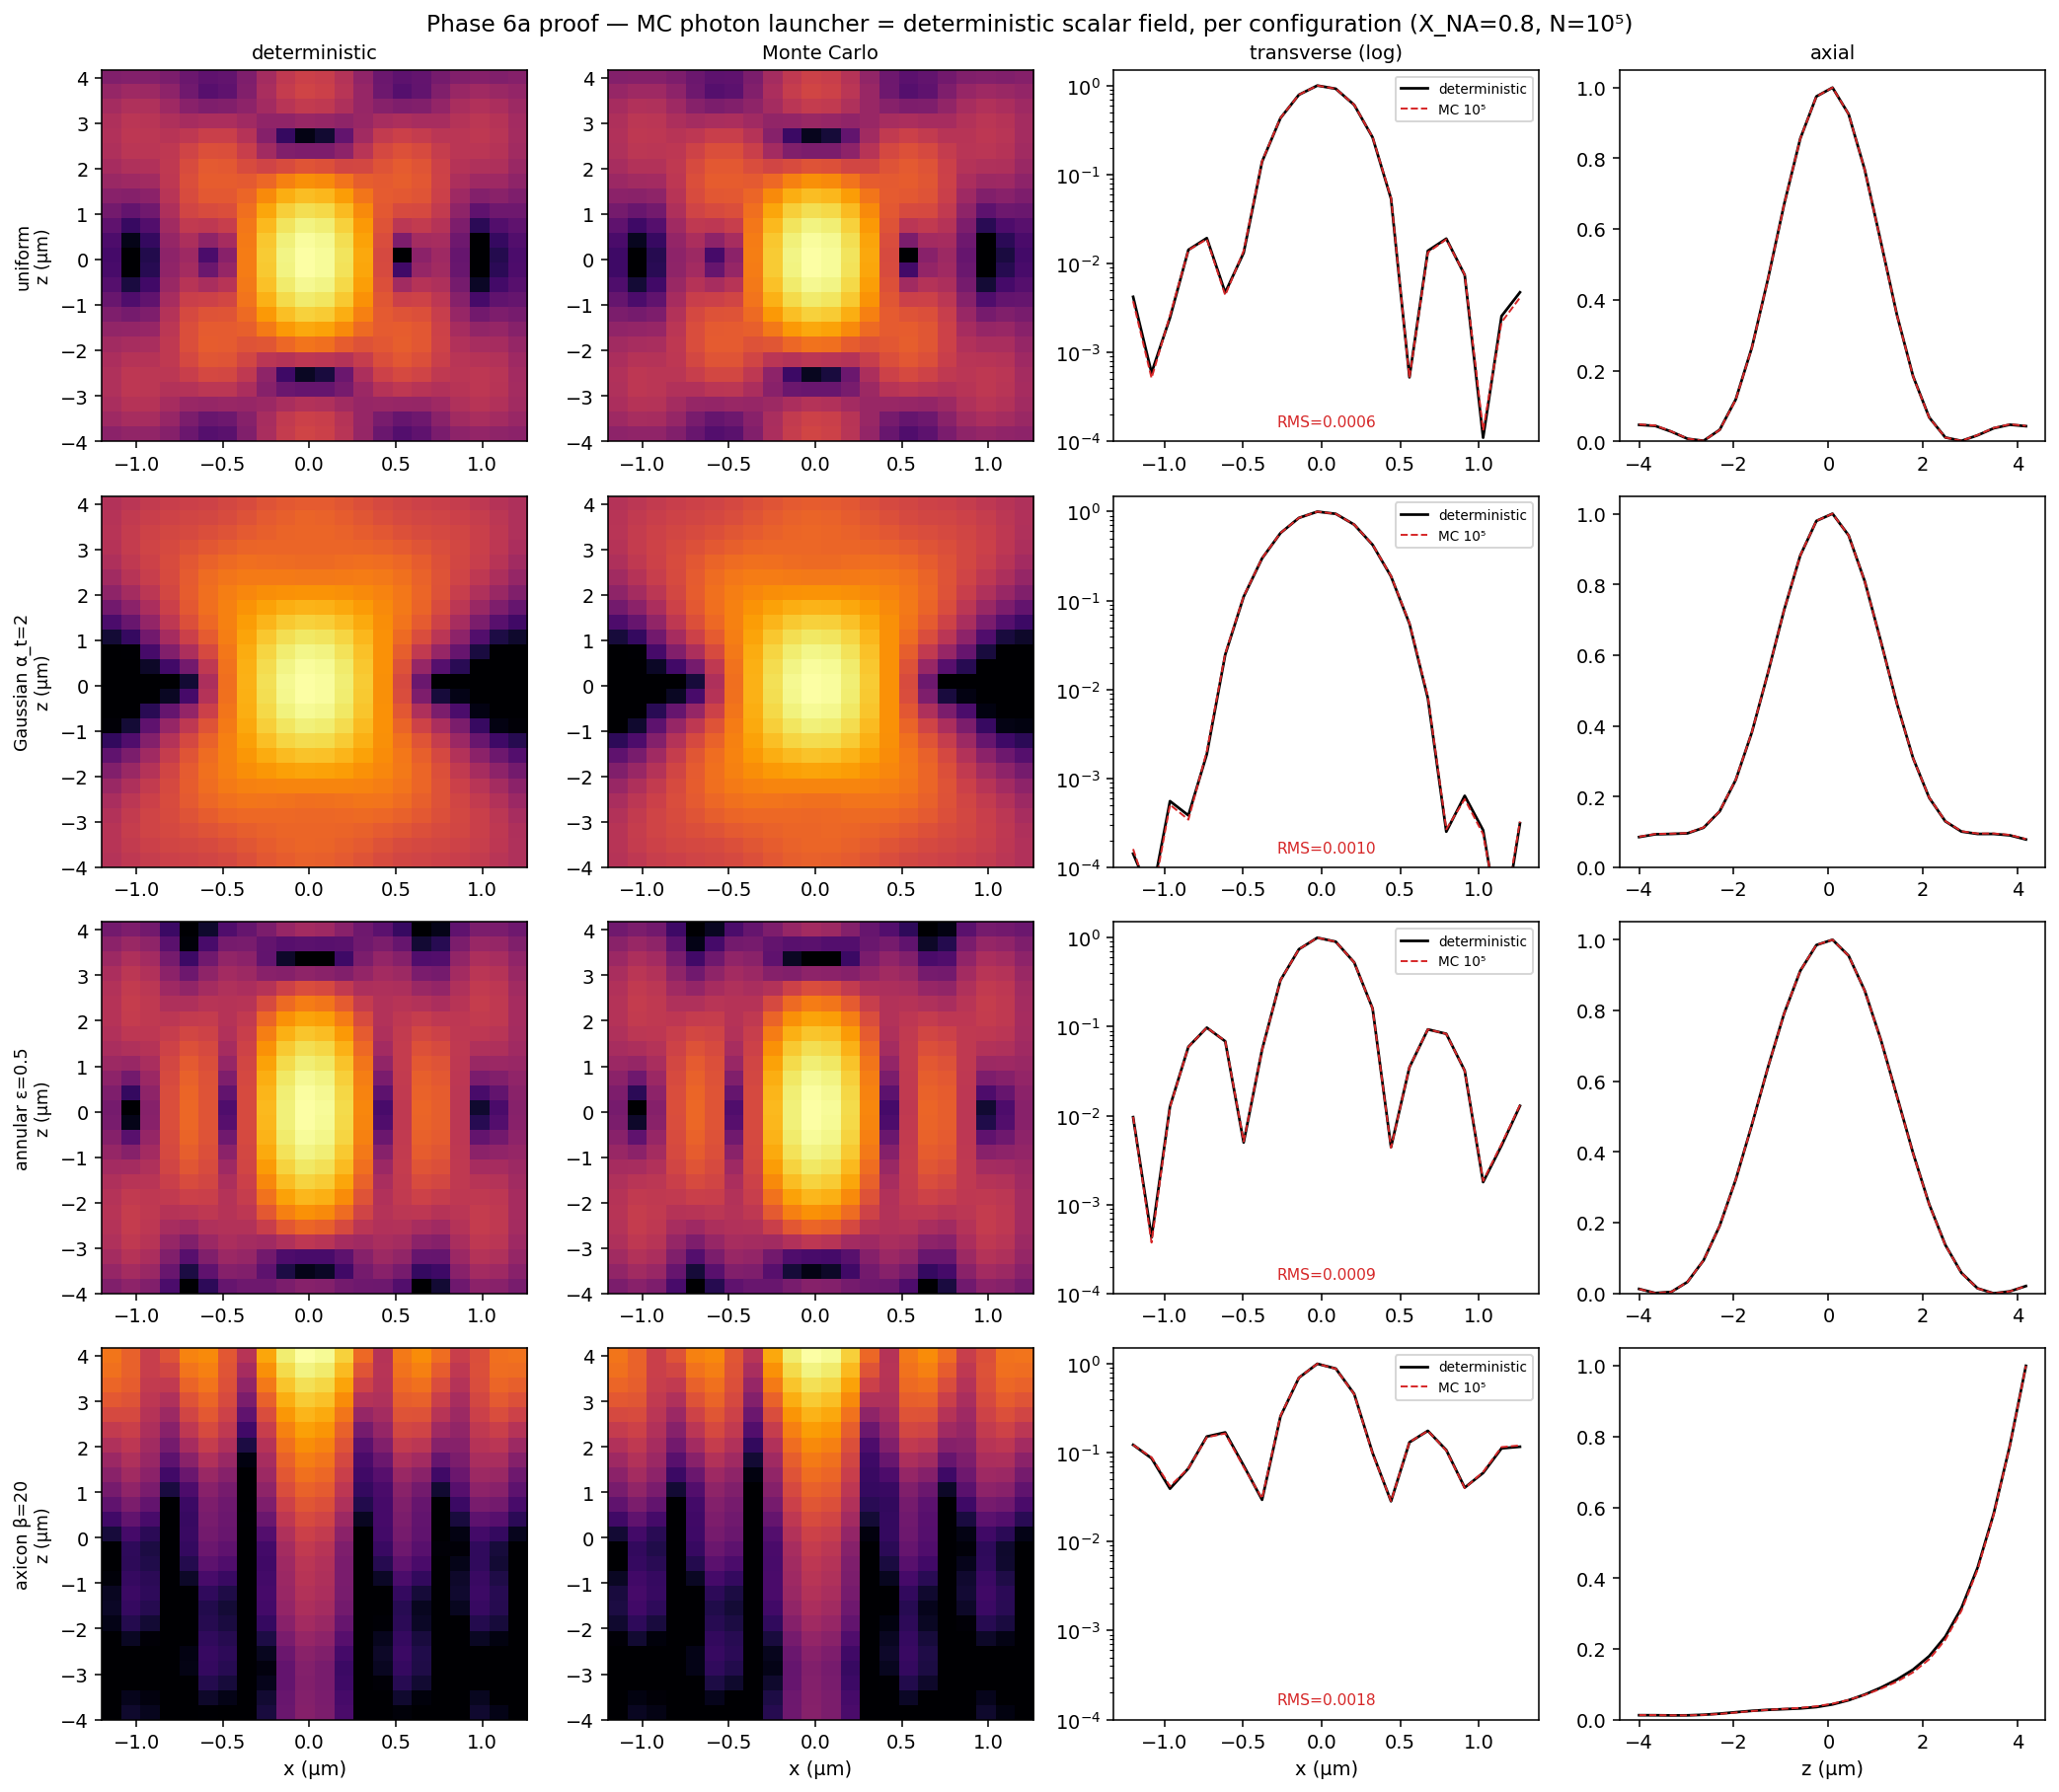
\includegraphics[width=0.9\textwidth]{verify_mc_configs.png}\end{center}

\section*{3. Vector field}
Photons carry the refracted 3-vector polarization (Novotny--Hecht Eq.~3.66);
$|E_x|^2+|E_y|^2+|E_z|^2$ reproduces both Richards--Wolf cuts ($|I_0-I_2|^2$ on
the $y$-axis, $|I_0+I_2|^2+4|I_1|^2$ on the $x$-axis), RMS $\sim6\times10^{-4}$.
\begin{center}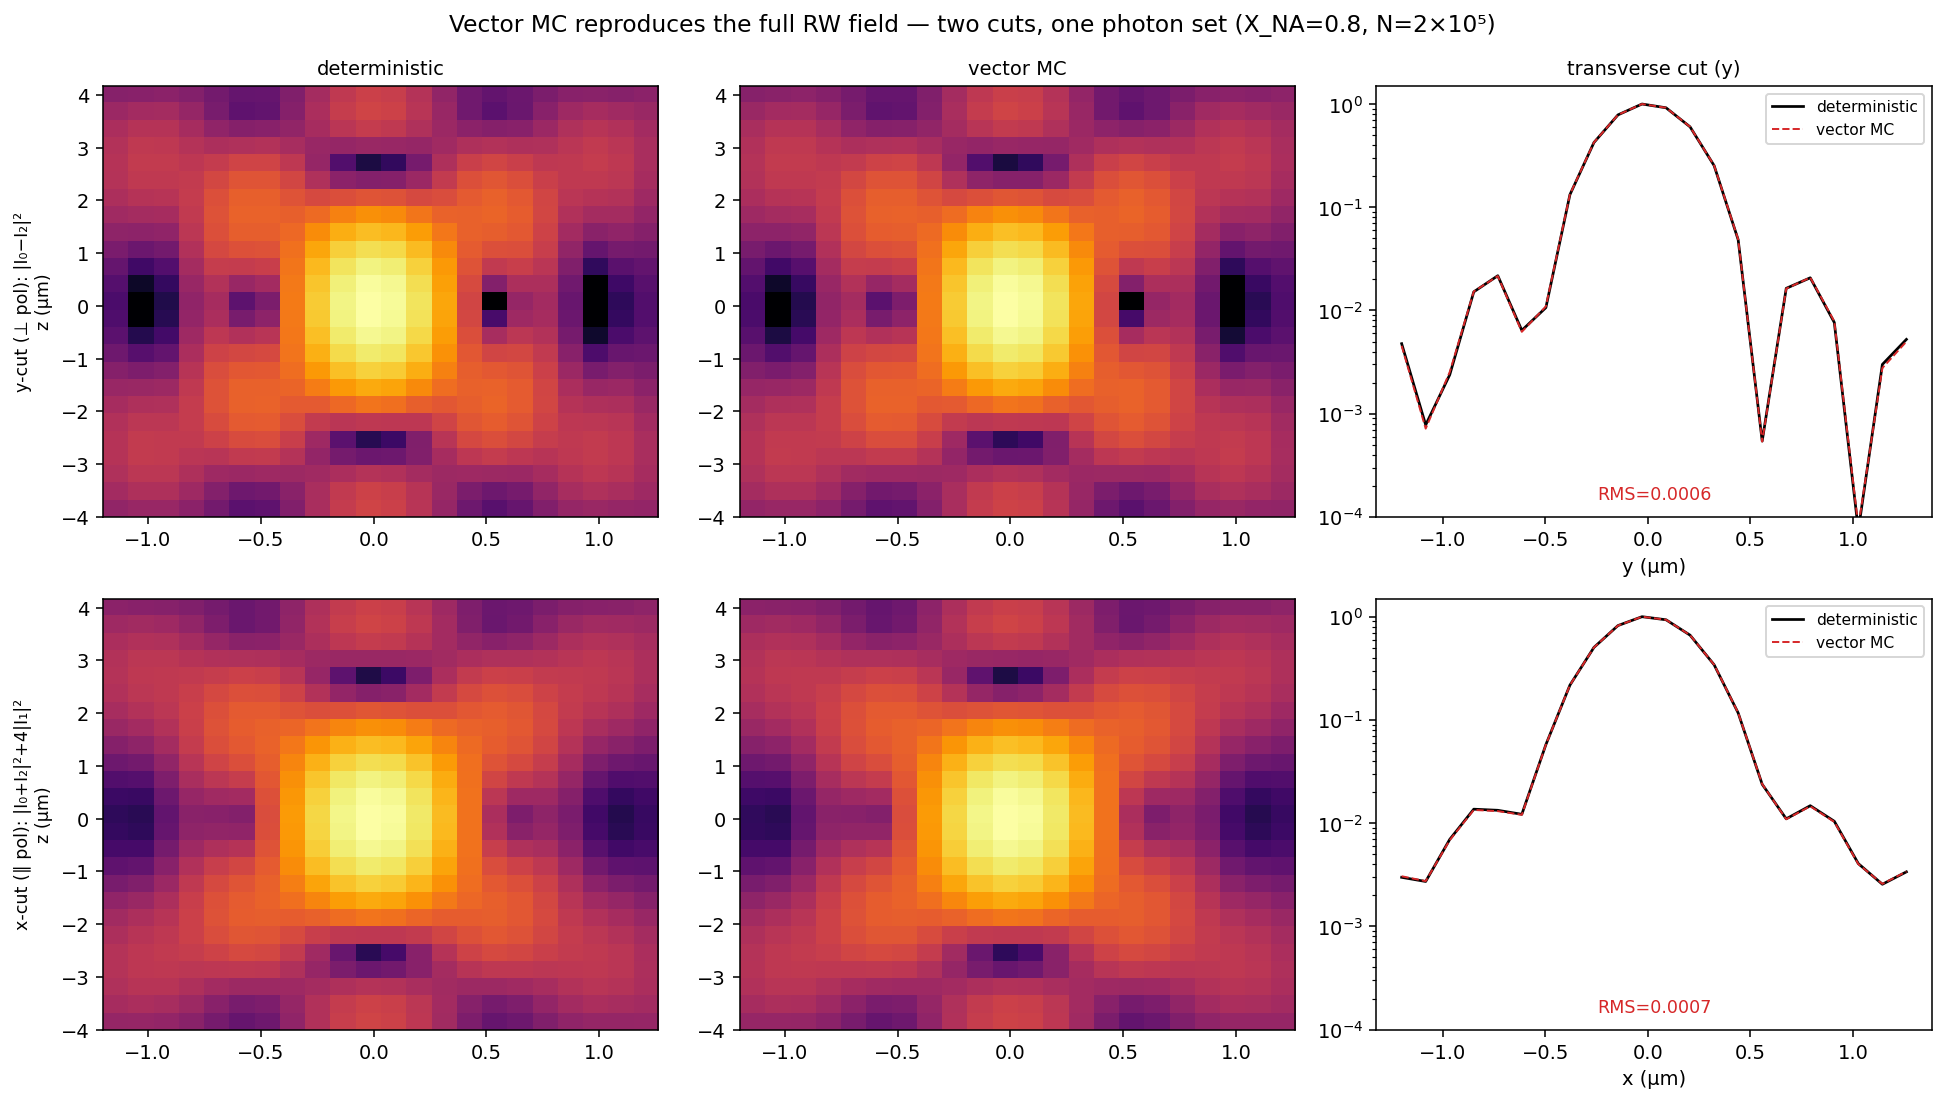
\includegraphics[width=0.9\textwidth]{verify_mc_vector.png}\end{center}

\section*{4. Sampling requirements --- sufficient $N$ and voxel size}
Two \emph{independent} requirements. \textbf{(A) Sufficient $N$} (statistical):
RMS $\propto 1/\sqrt N$, null floor $\propto 1/N$; $N\approx3\times10^3$ for 1\%
RMS, axicon needs $\approx10^4$ for clean zeros. \textbf{(B) Voxel} (Nyquist on
the \emph{intensity}, twice the field frequency):
$dx=dy\le\lambda/(4\,\mathrm{NA})=234$~nm, $dz\le\lambda/(4n(1-\cos\alpha))=681$~nm;
we run at half (117 / 341~nm). FWHM recovery (normalised) is flat below the
Nyquist voxel and degrades above it.
\begin{center}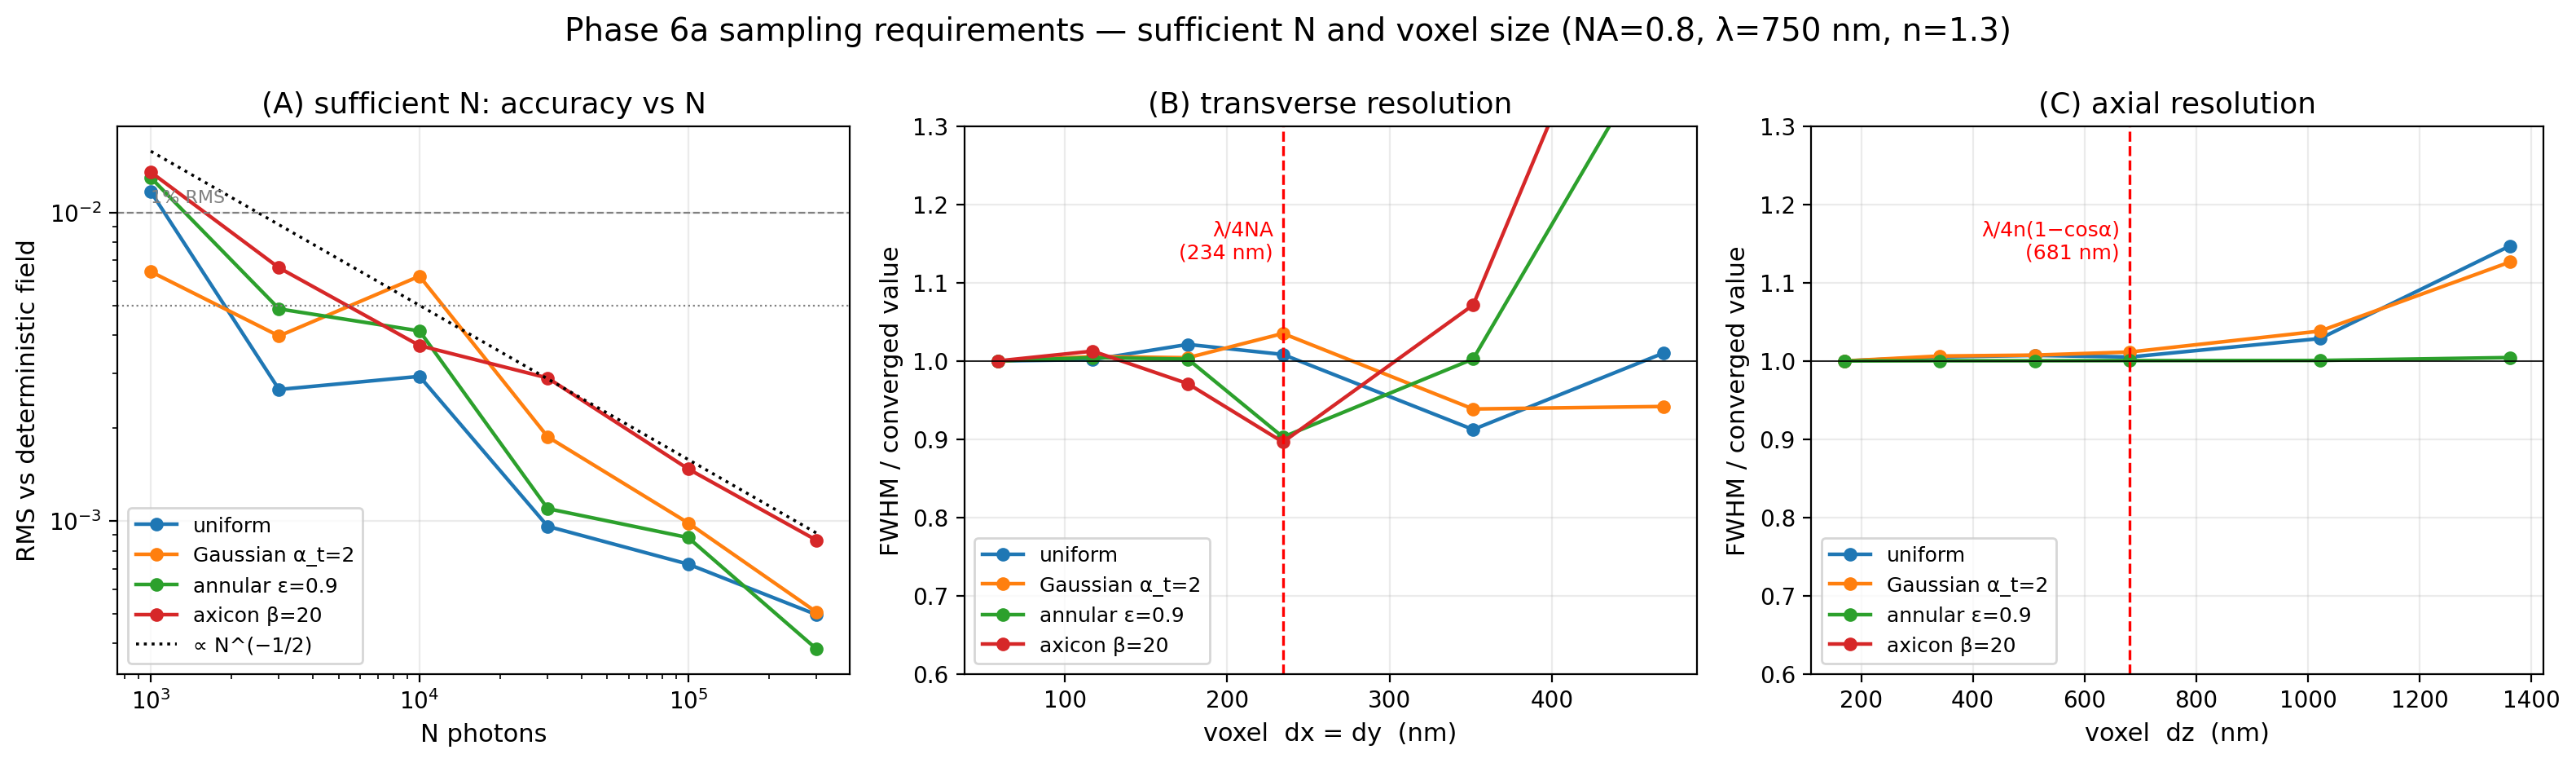
\includegraphics[width=0.99\textwidth]{study_sampling.png}\end{center}

\section*{5. Launcher initialization proof (the pre-scattering prerequisite)}
\textbf{Why correct from first principles}, not just distribution-matching: the
plane-wave decomposition \emph{is} Debye--Wolf theory; directions are confined
to the cone $\theta\le\alpha$ ($\sin\alpha=\mathrm{NA}/n$) with statistical
weight $A(\theta)\sqrt{\cos\theta}$ fixed by the input illumination $\times$ the
aplanatic (Abbe sine) factor --- energy conservation, not a fit. Location and
direction are locked by $\rho=f\sin\theta$, and the importance-sampling estimator
is provably unbiased, so $N\to\infty$ convergence is guaranteed \emph{before}
running. In the clear medium photons travel in straight lines (the wavefront
normals).

\textbf{Distribution} (uniform \& Gaussian $\alpha_t=2$): (1) sampled $\theta$
matches the Debye--Wolf density $|A|\sqrt{\cos\theta}\sin\theta$, KS
$=0.0009\approx1/\sqrt N$; (2) $\varphi$ uniform (flatness 0.025; both inputs
coincide); (3) recovered $A(\theta)$ flat / Gaussian; (4) recovered radial input
intensity $|A|^2$ = flat disk / Gaussian spot.
\begin{center}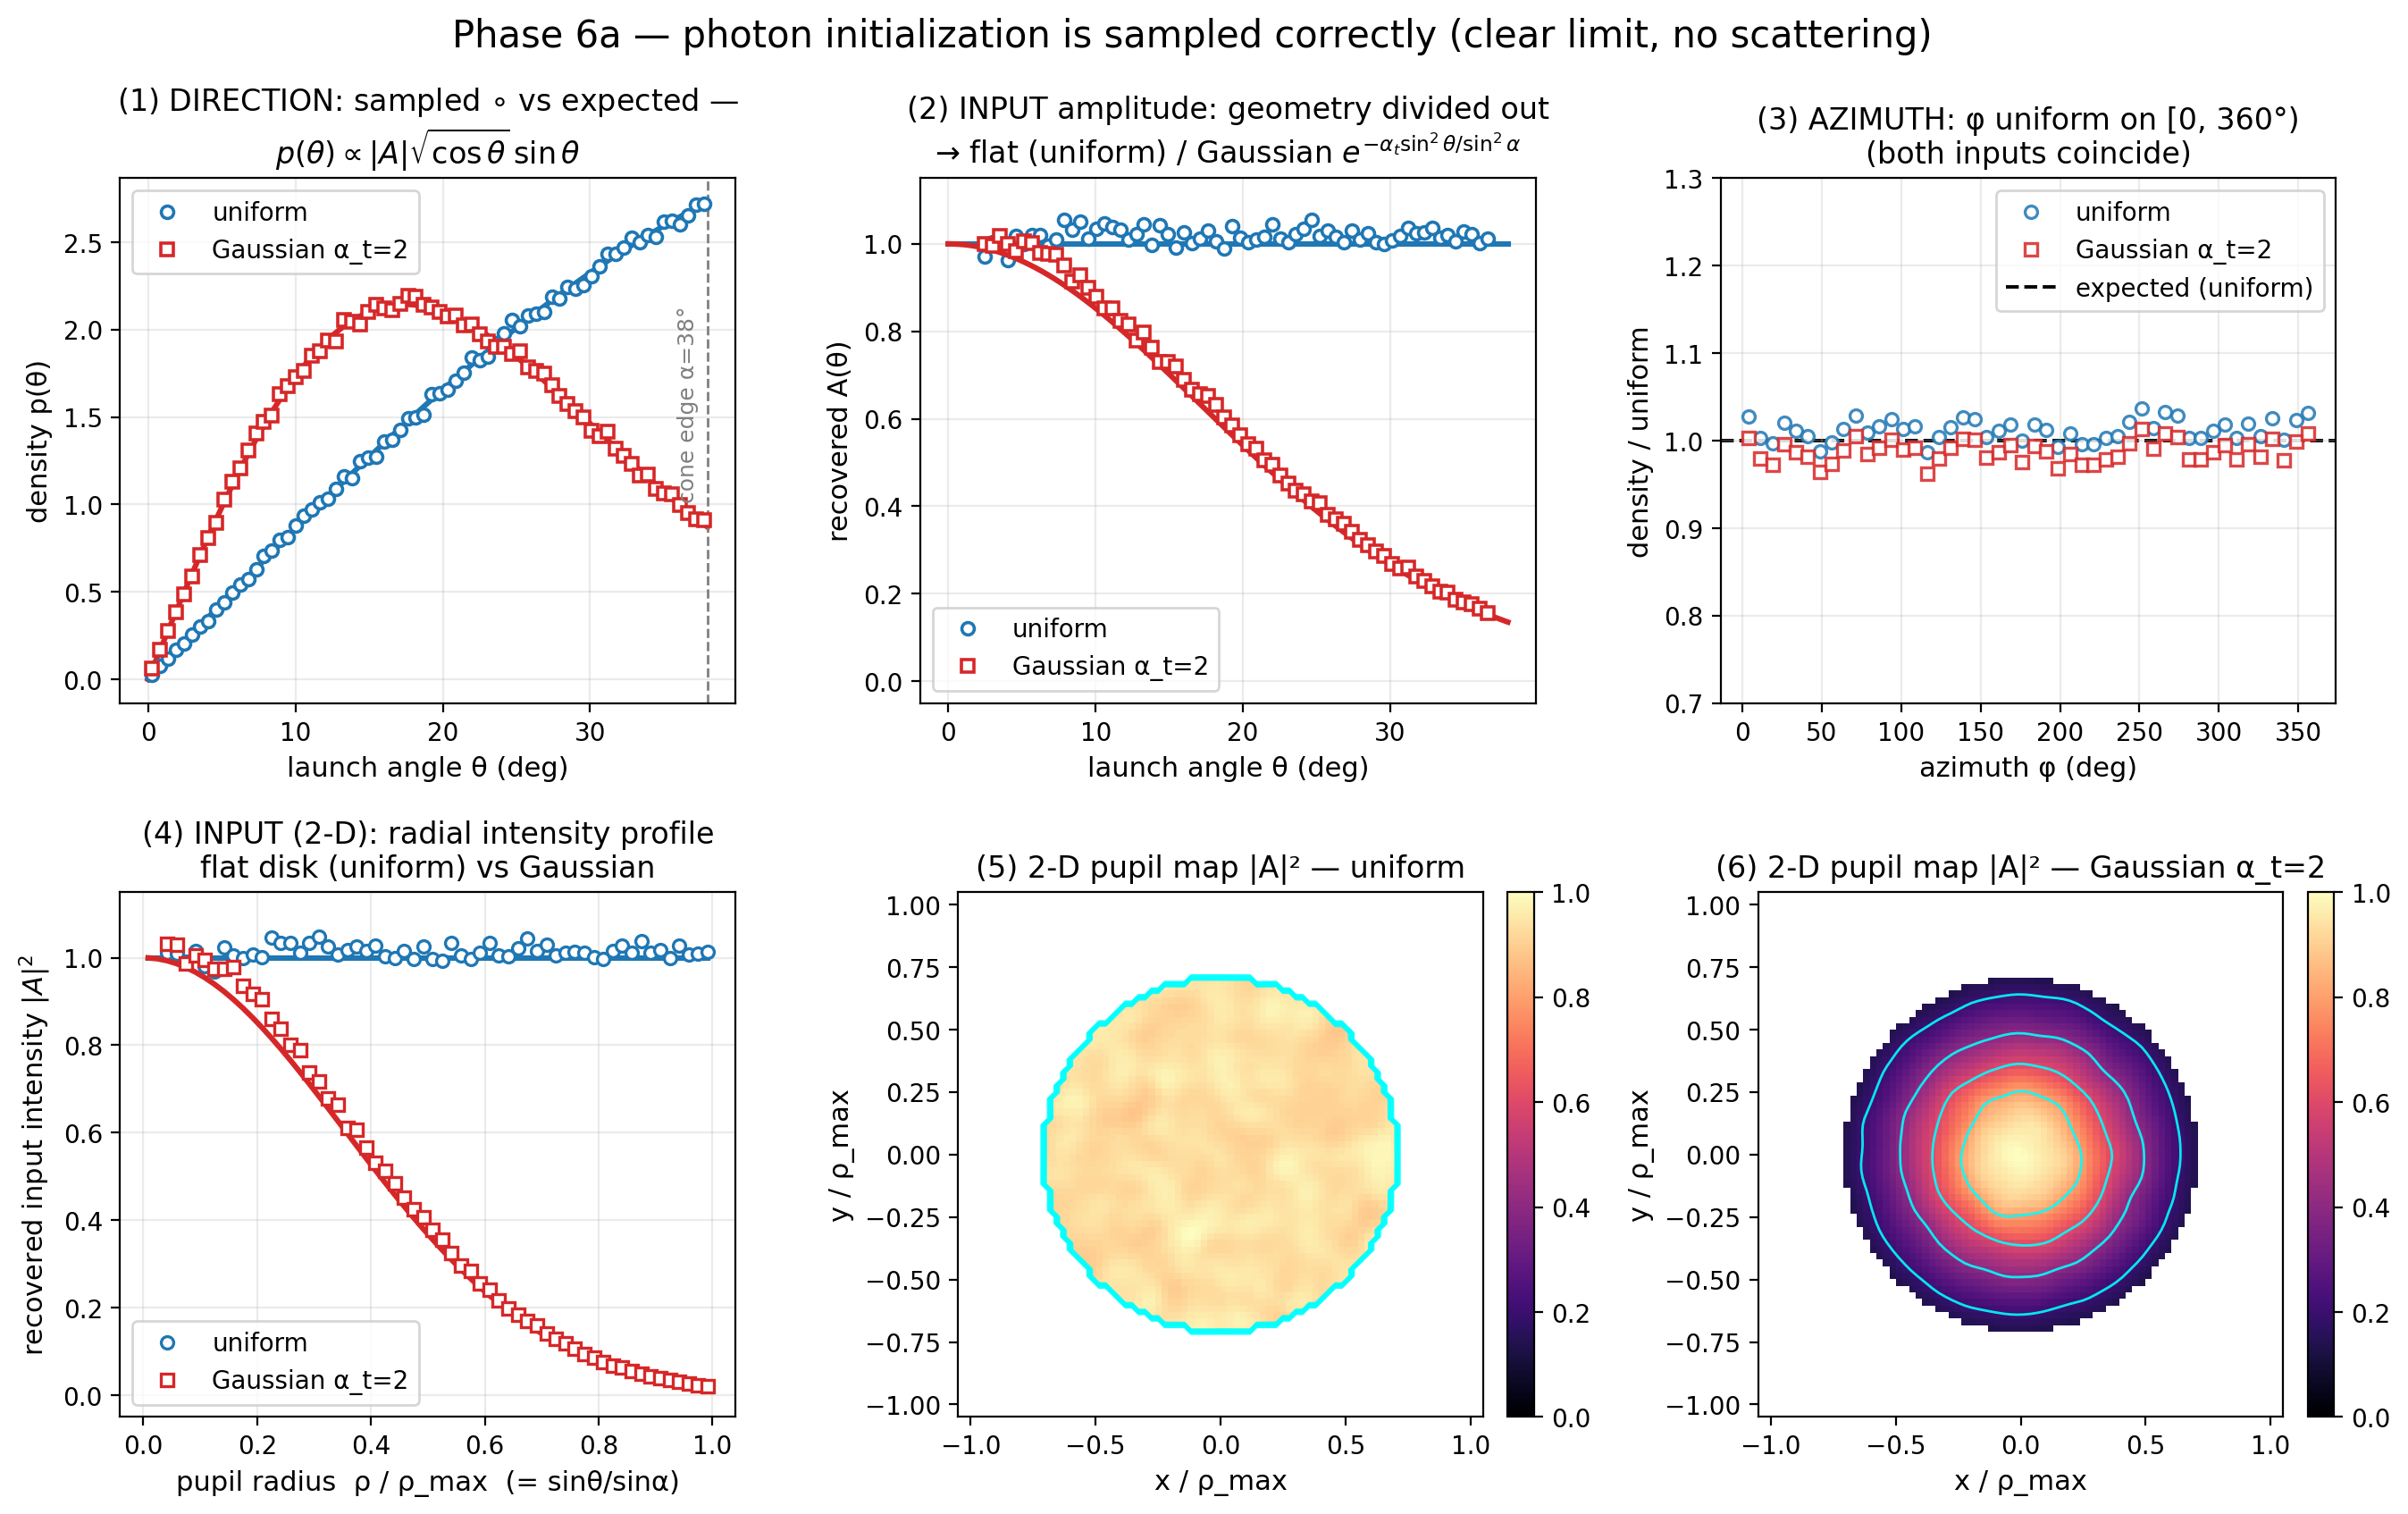
\includegraphics[width=0.99\textwidth]{verify_launcher.png}\end{center}
\textbf{Intensity}: MC matches the deterministic field on transverse \& axial
cuts (through peak, zeros, side-lobes) and on the $x$--$z$ slice, RMS
$0.0006$--$0.0008$; the deterministic iso-value contours sit on the MC heat map.
\begin{center}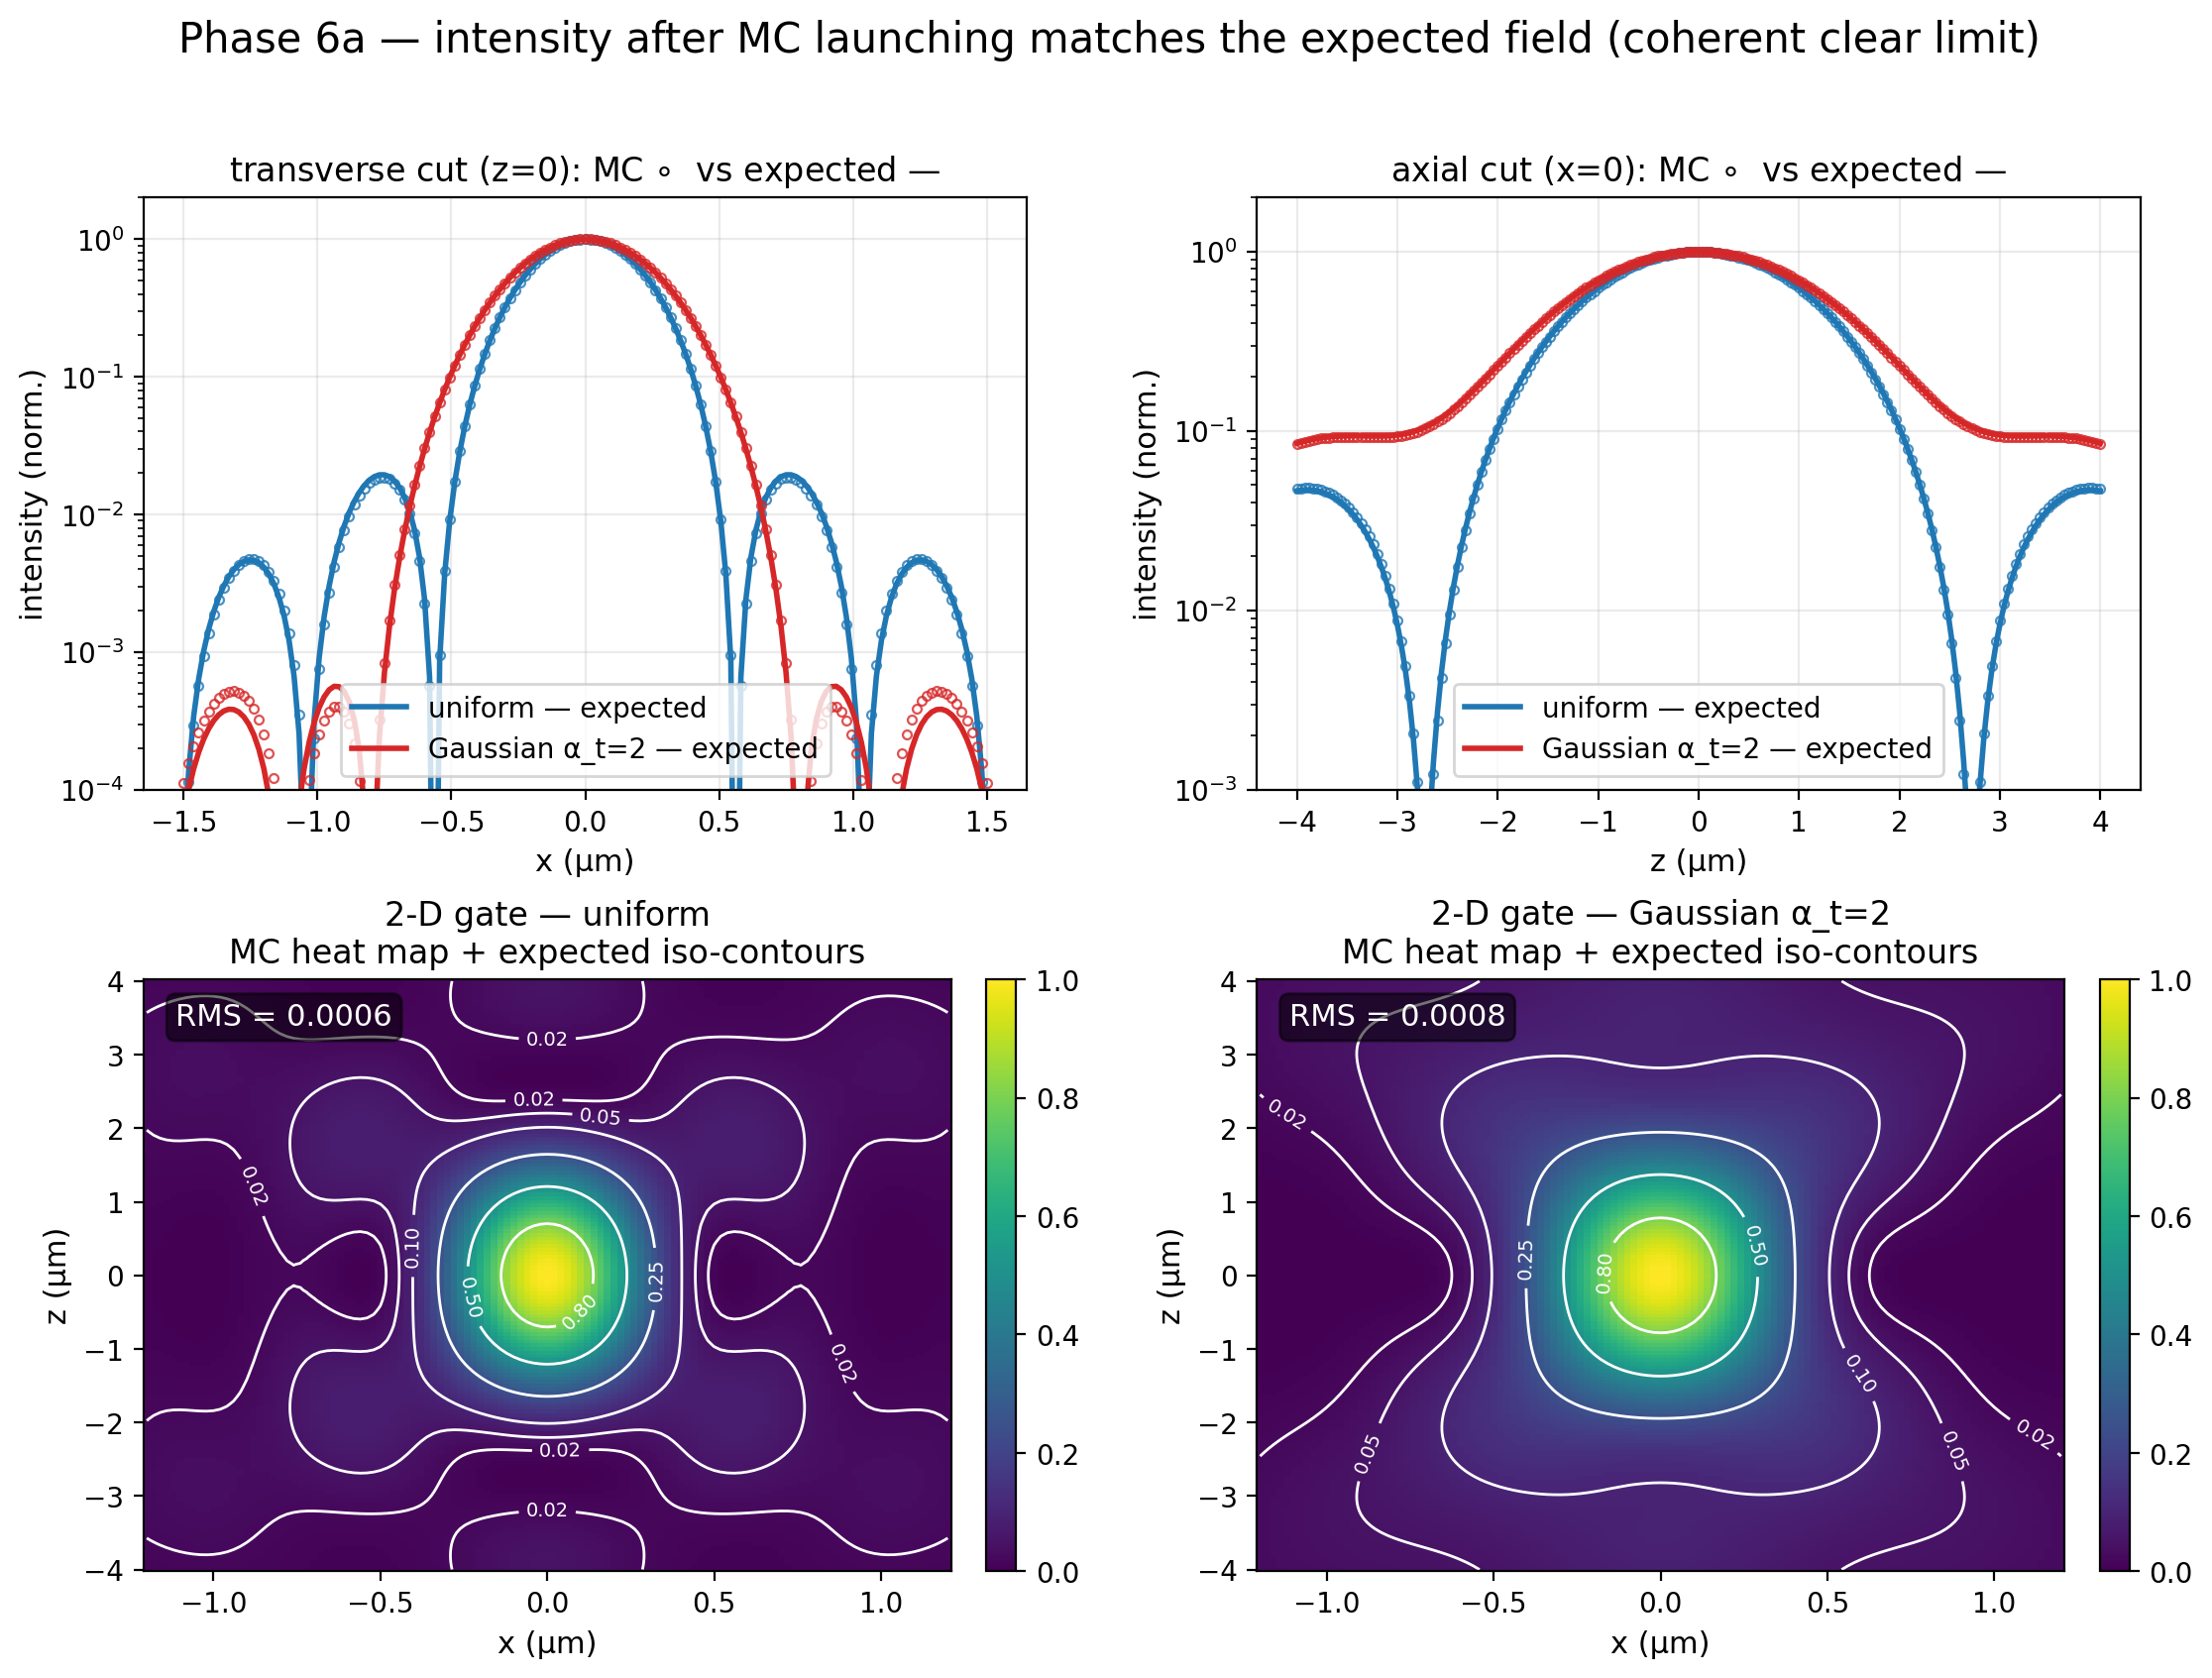
\includegraphics[width=0.99\textwidth]{verify_launcher_intensity.png}\end{center}

\section*{6. Optional parallelism}
Partitioning photons across workers and summing the partial complex fields is
identical to serial (the field is an additive sum): agreement to FP round-off
($8.7\times10^{-16}$ relative), speedup $1.7/2.9/3.6\times$ at 2/4/8 jobs.
\begin{center}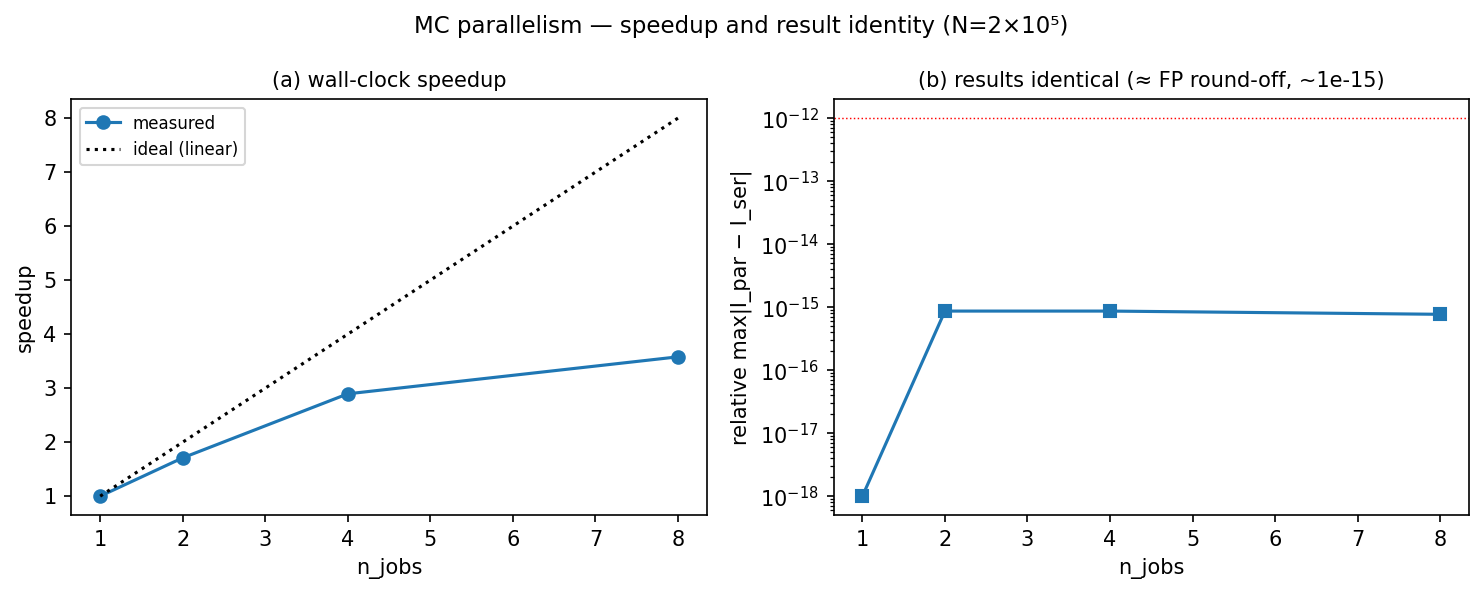
\includegraphics[width=0.78\textwidth]{profile_parallel.png}\end{center}

\section*{7. Scattering kernel --- pre-validated; 6b next}
The kernel for the next phase is already checked in isolation: Henyey--Greenstein
$\langle\cos\theta\rangle=g$; isotropic $\langle\mu_z^2\rangle=1/3$; unit-norm
directions; Beer--Lambert ballistic fraction
$\exp(-\mu_s L)=0.607/0.367/0.135/0.018$ exact.
\begin{center}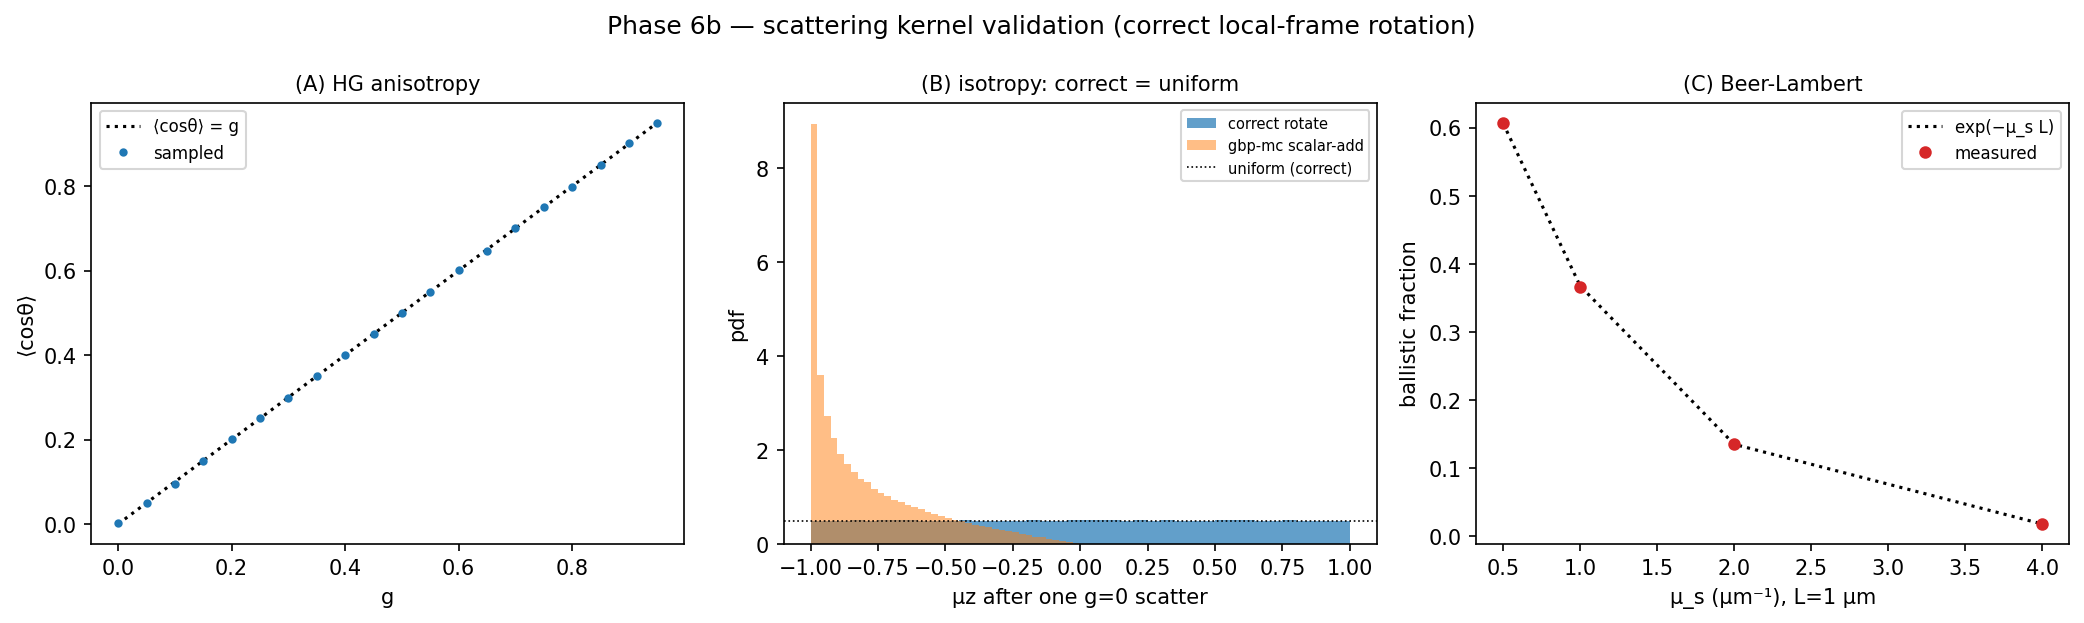
\includegraphics[width=0.9\textwidth]{verify_scatter_kernel.png}\end{center}
\textbf{6b note.} Because the launcher is certified, the only new physics is
attenuation: the ballistic (coherent) field attenuates in \emph{amplitude} as
$\exp(-\mu_s L/2)$ (Beer--Lambert $\exp(-\mu_s L)$ in intensity), with the
scattered energy forming a separate \emph{incoherent} halo. $\mu_s\to0$ recovers
Phase 6a by construction.

\section*{8. Addenda --- statistical spread, wavelength MC, photon budgets}
\textbf{Statistical spread} (\texttt{mc\_variance.png}): per-point mean $\pm1\sigma$
over $K{=}40$ runs (transverse \& axial, $N$=2k/20k); the band is widest in the
dark side-lobes/zeros and shrinks $\propto1/\sqrt N$.
\begin{center}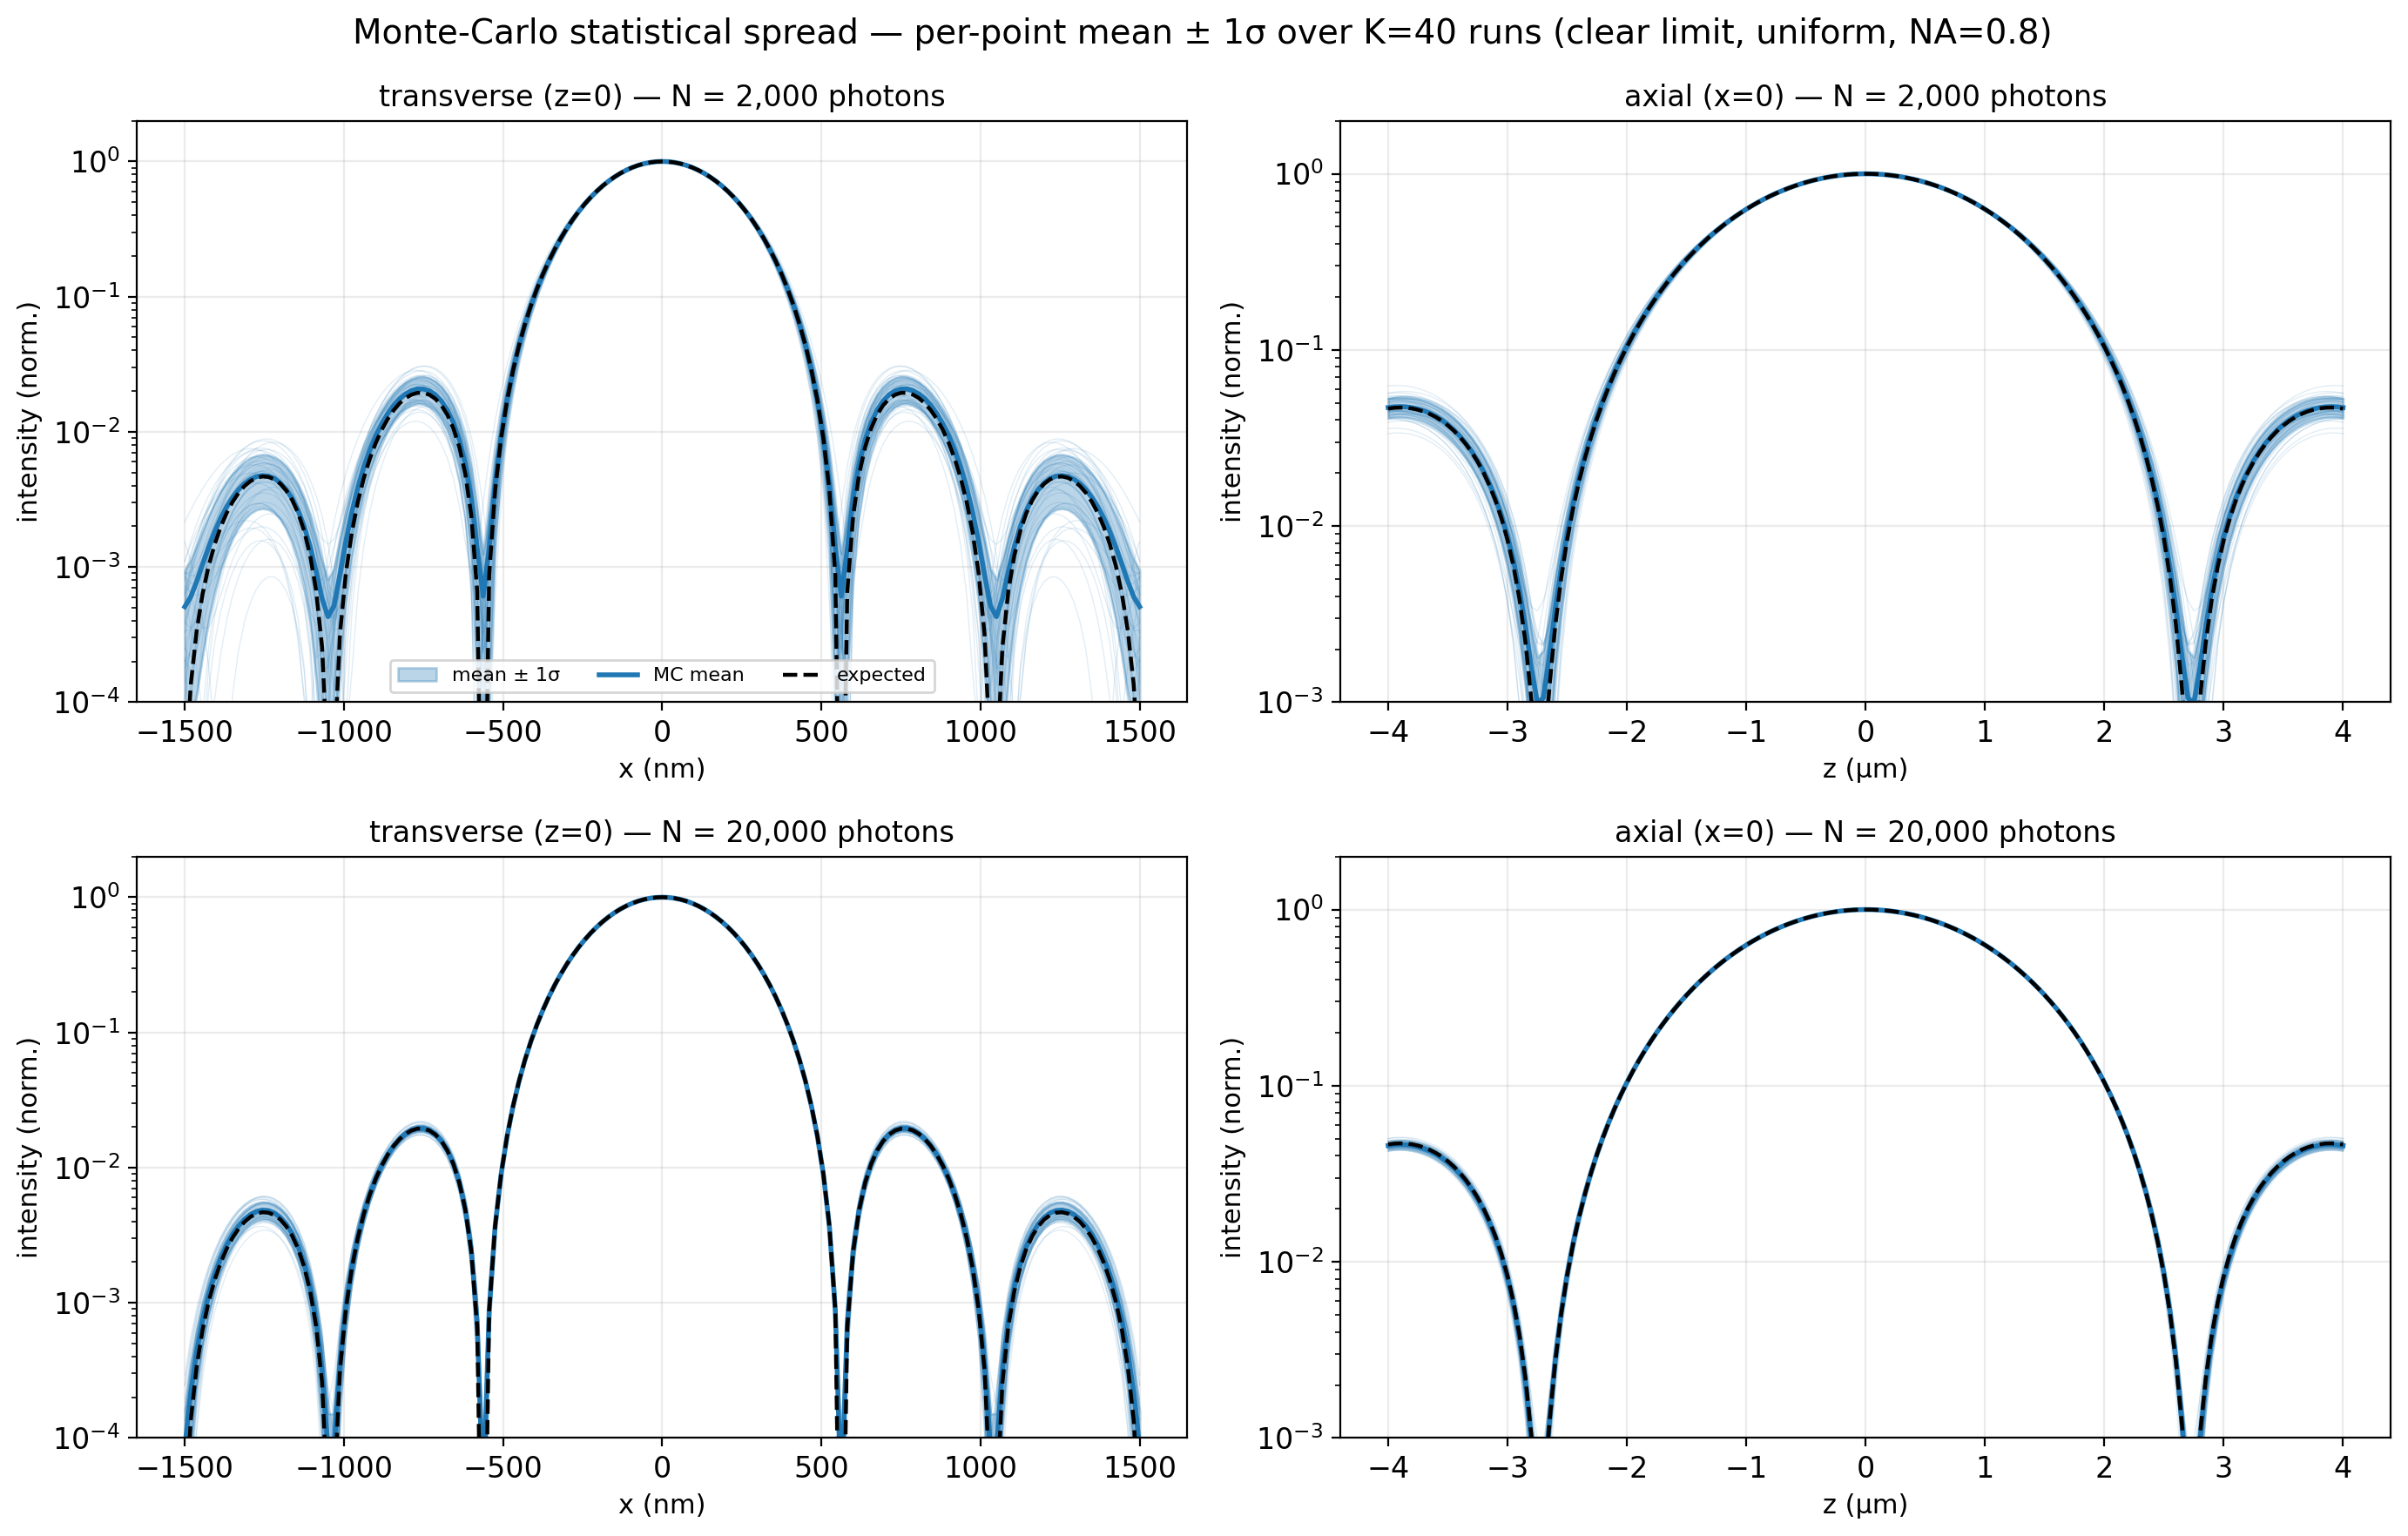
\includegraphics[width=0.84\textwidth]{mc_variance.png}\end{center}

\textbf{Per-photon wavelength MC} (\texttt{verify\_mc\_pulsed.png}): drawing each
photon's $\lambda\sim|E(\omega)|^2$ (coherent within a wavelength, incoherent
across) reproduces the deterministic Eq.~10 to RMS $3$--$5\times10^{-4}$ and fills
the CW zeros. Use it for pulsed light in \emph{scattering} media (each $\lambda$
sets its own $\mu_s$); the deterministic sum is cheaper in a clear medium.
\begin{center}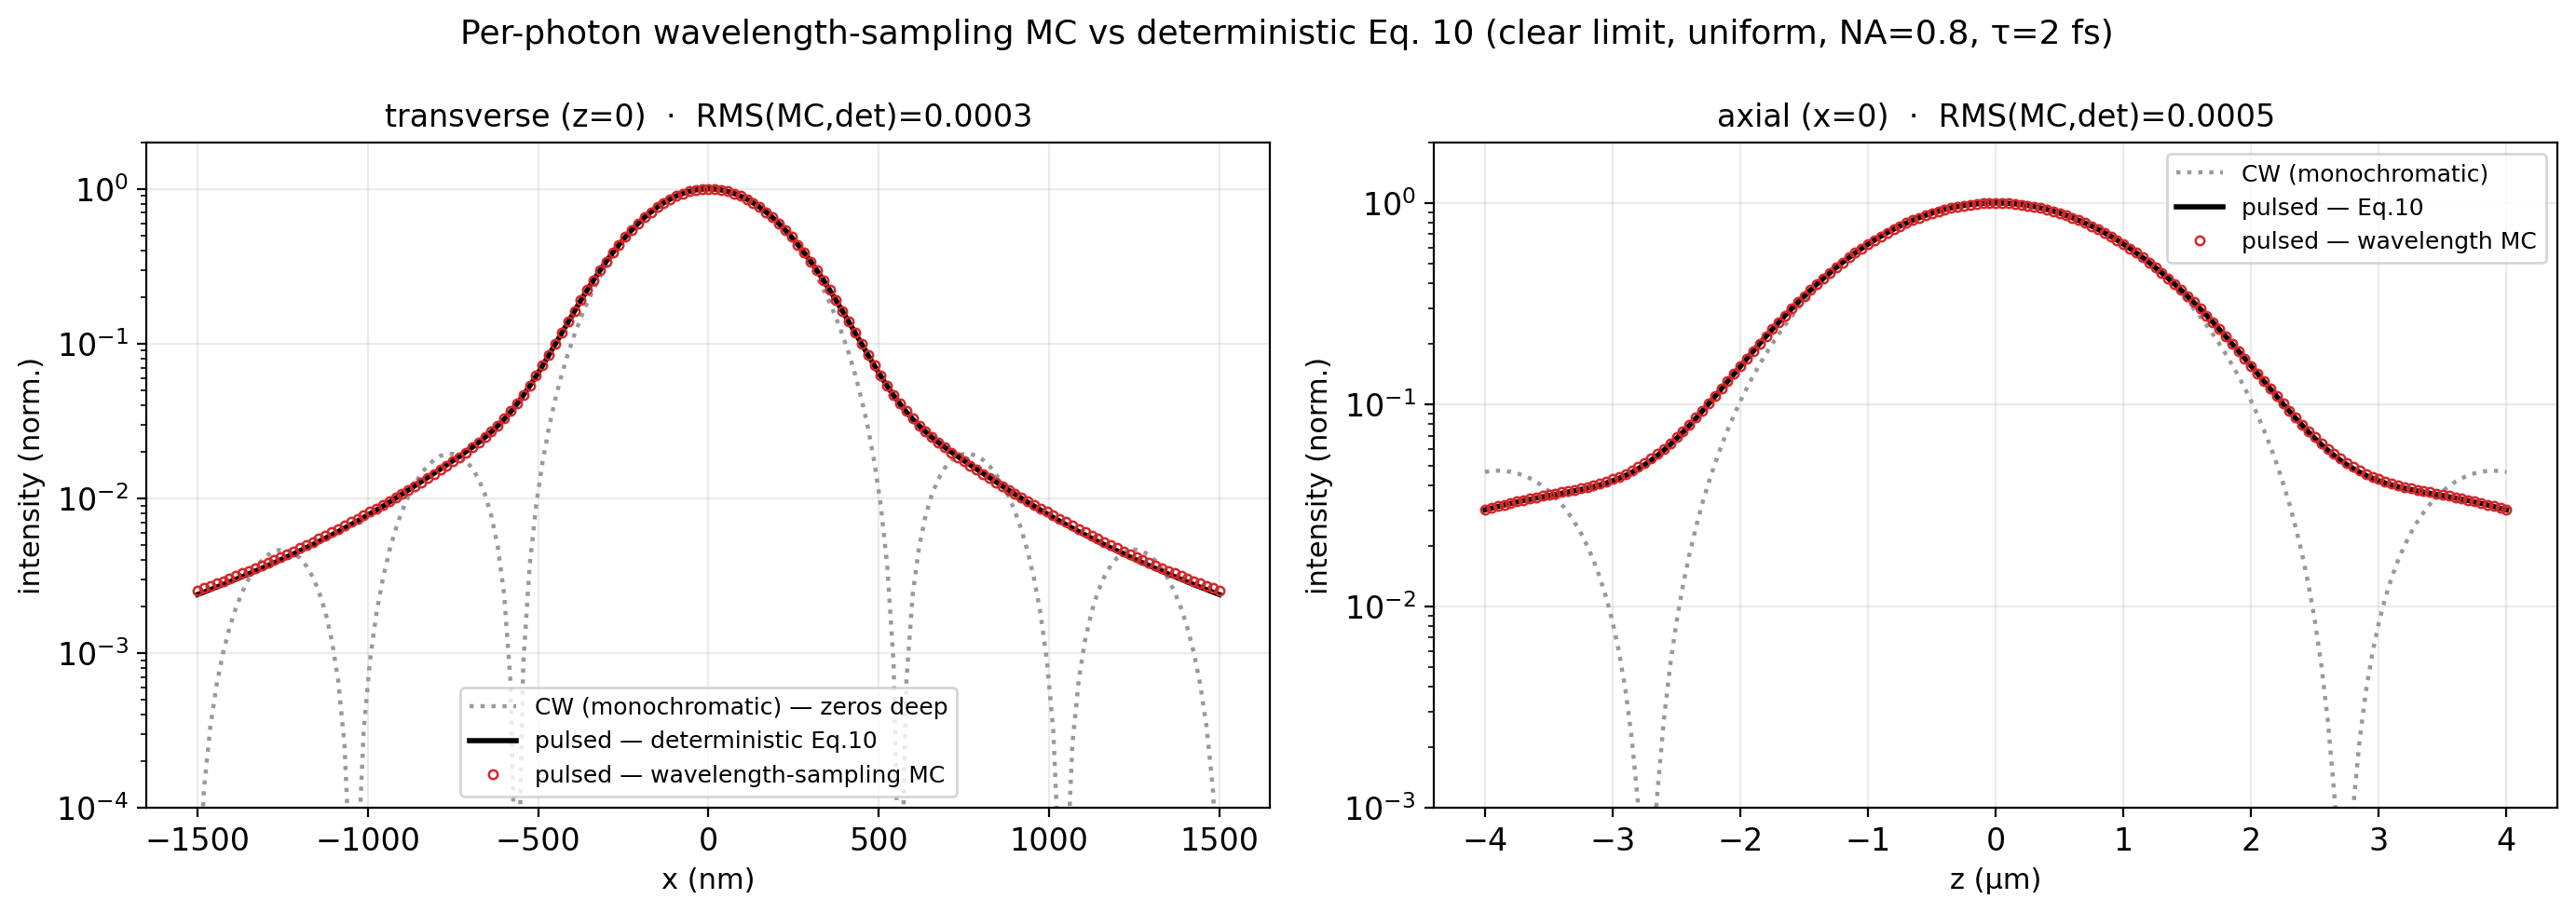
\includegraphics[width=0.99\textwidth]{verify_mc_pulsed.png}\end{center}

\textbf{Photons per model} (\texttt{photons\_per\_model.png}): $N$ for 1\% RMS ---
NA 0.1--1.2 $\sim$200--2100; Gaussian $\alpha_t$ 0$\to$4 $\sim$0.9k$\to$2.4k;
annular $\varepsilon$ 0$\to$0.99 $\sim$0.9k$\to$1.3k; axicon $\beta$=0/5/10 $\sim$0.9k
but $\beta$=20 $\approx$40k and $\beta$=40 $\approx$370k. The cost is set by how fast
the pupil \emph{phase} winds (coherent cancellation), not by NA --- and in the
clear limit it is small because this is importance-sampled coherent quadrature of
a smooth 2-D integral. Scattering (high-dimensional path space, an incoherent
halo over many voxels, an exponentially small ballistic fraction at depth) is
what pushes counts to the usual $10^6$--$10^8$.
\begin{center}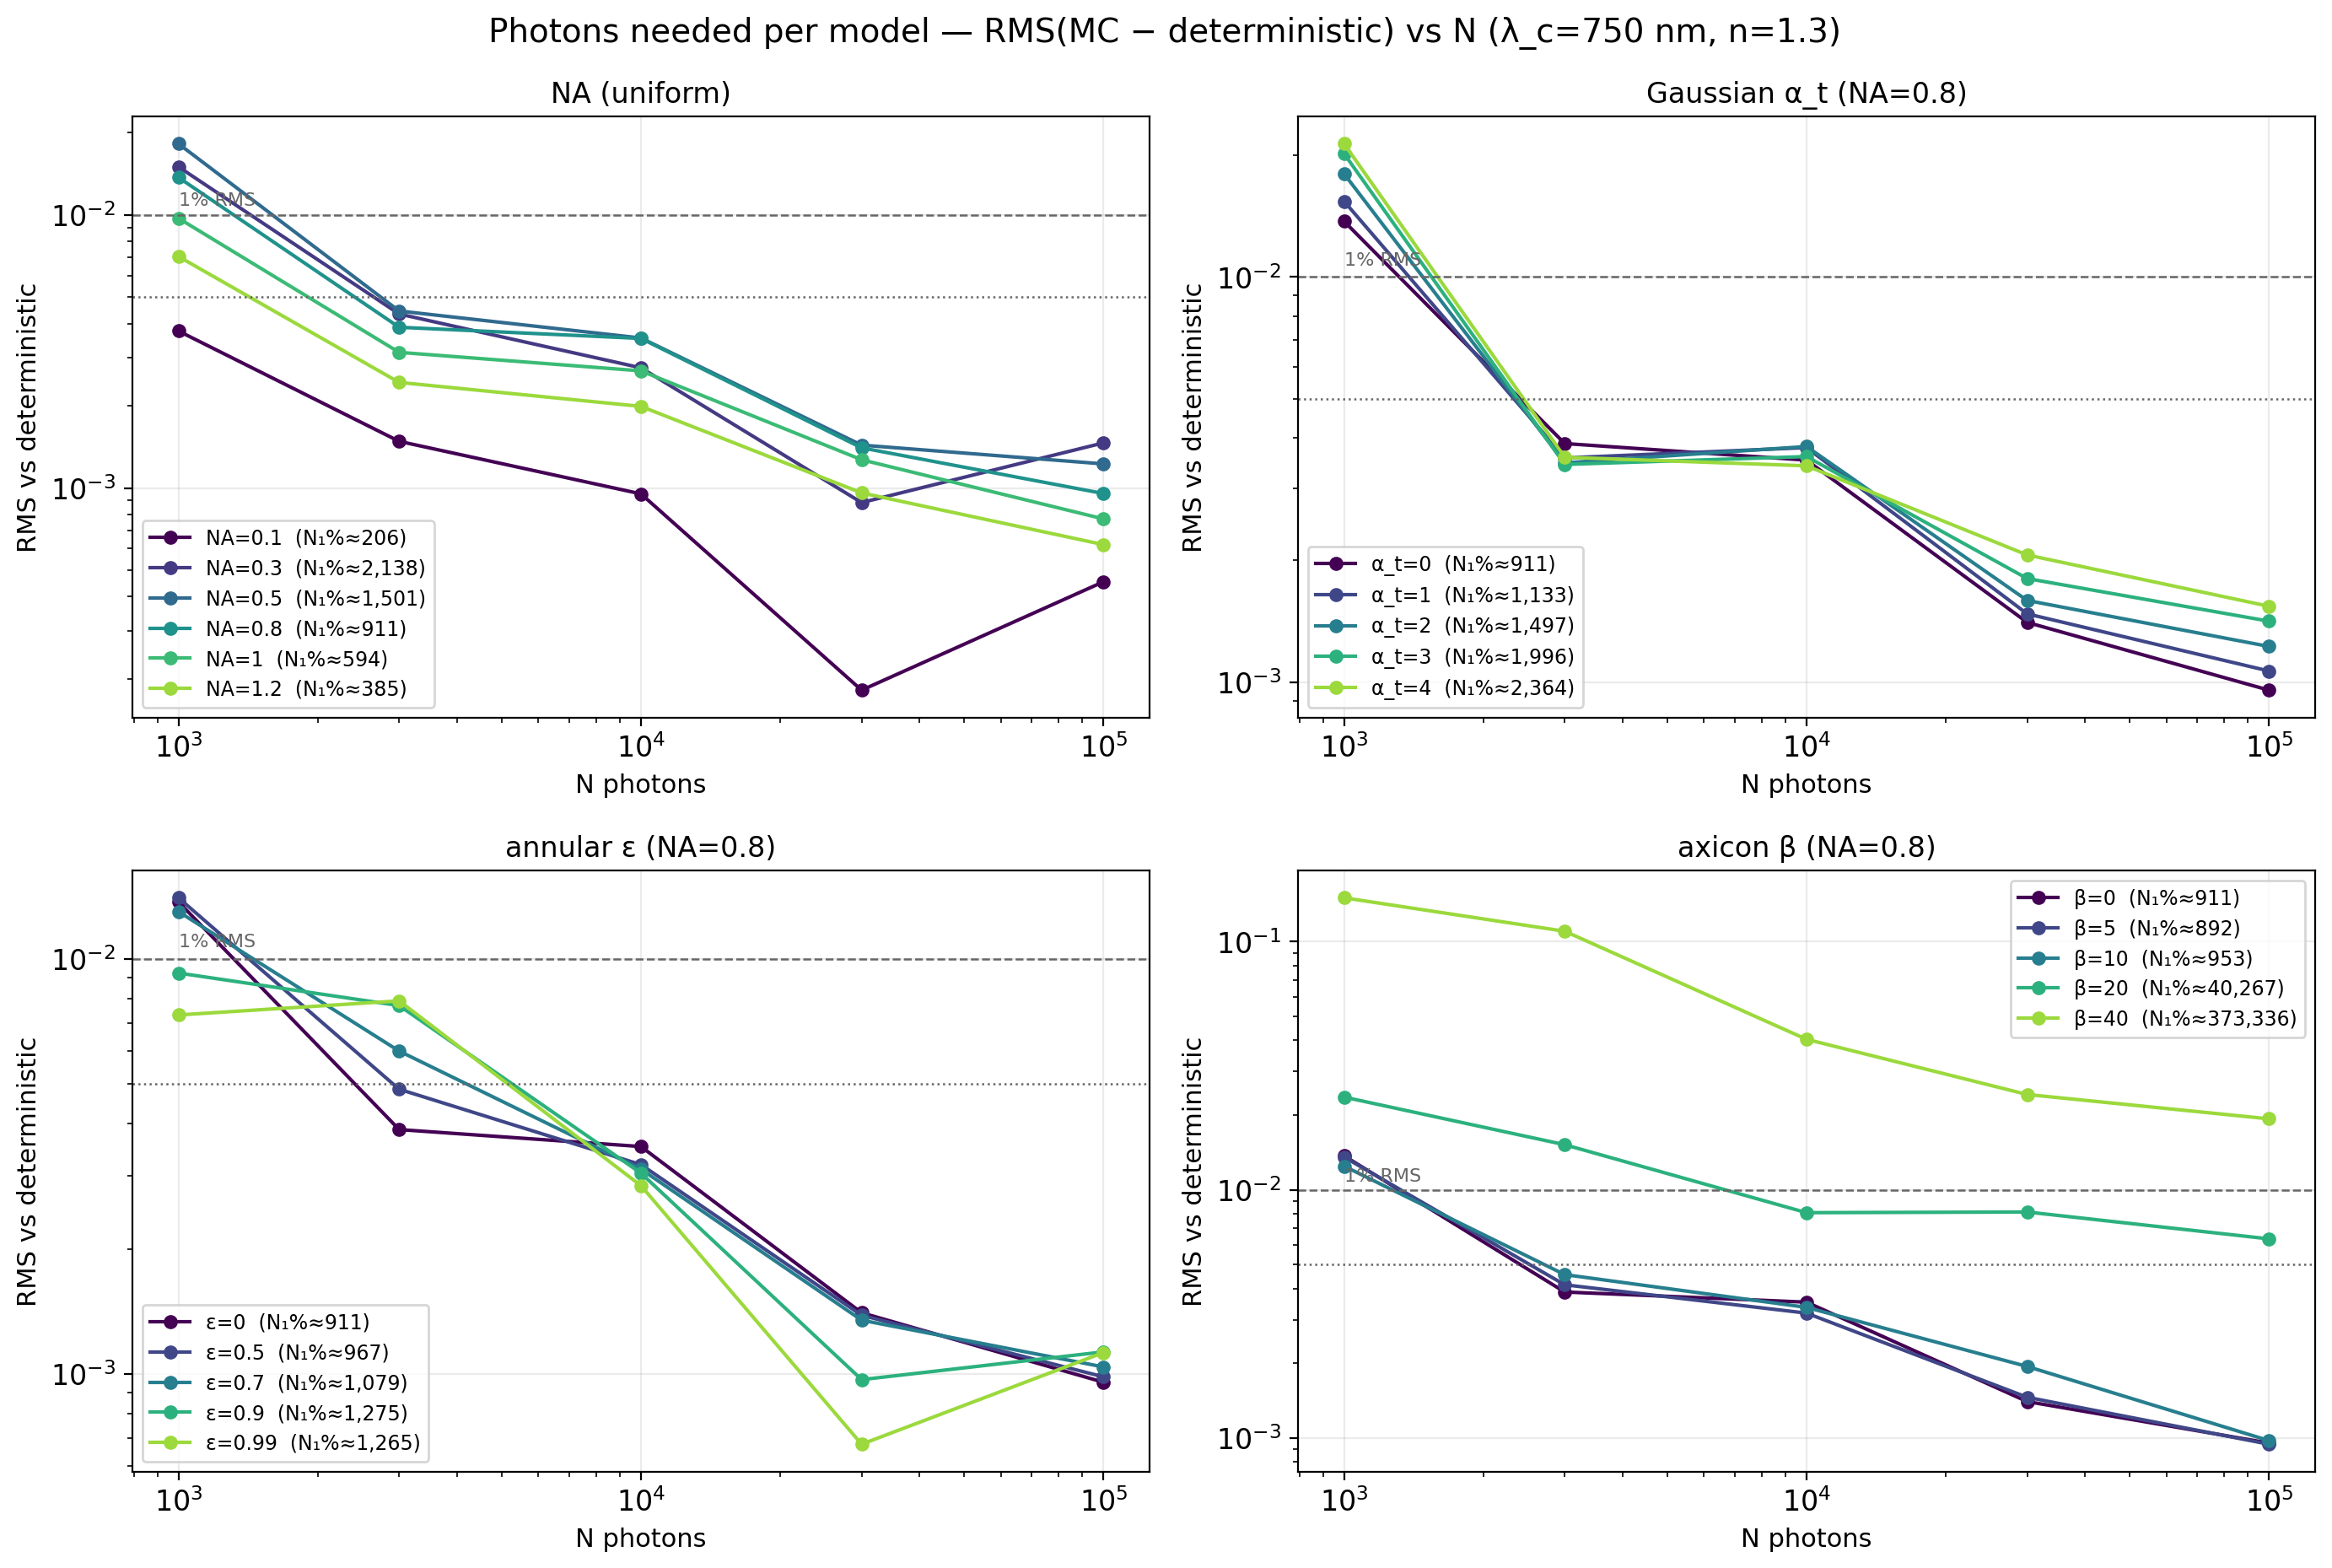
\includegraphics[width=0.99\textwidth]{photons_per_model.png}\end{center}

\section*{9. Phase 6b --- focused beam through a scattering slab (first run, validated)}
Slab $z\in[-d,0]$ (focus at the back face), $d=20$~µm, $g=0.9$, NA=0.8, $K=10$
trials. Each photon is the converging ray, entering at
$(-d\tan\theta\cos\varphi,-d\tan\theta\sin\varphi,-d)$. The focal field splits
into a \textbf{ballistic coherent core} (amplitude $e^{-\mu_s L/2}$,
$L=d/\cos\theta$) and a \textbf{diffuse incoherent halo} (forward-scattered
photons, Henyey--Greenstein walk). \emph{All three validation rungs pass}:
\begin{itemize}\itemsep1pt
\item \textbf{RUNG 1 continuity:} at $\mu_s=0$ the core $=$ the clear focus
  (peak ratio 1) and the halo $=0$.
\item \textbf{RUNG 2 Beer--Lambert:} the MC ballistic fraction equals the
  analytic cone average $\langle e^{-\mu_s d/\cos\theta}\rangle$ to $<0.001$
  across $\tau=\mu_s d \in[0,4]$.
\item \textbf{RUNG 3 energy:} ballistic $+$ forward $+$ back $+$ absorbed $=1$ to
  $2\times10^{-16}$.
\end{itemize}
\textbf{Physics.} As $\tau$ grows the ballistic focus dims
($E_{\text{ball}}=0.89/0.57/0.33/0.011$ at $\tau=0.1/0.5/1/4$, \emph{below} the
normal-incidence $e^{-\tau}$ because $d/\cos\theta>d$), forward-scatter dominates
($g=0.9$; backscatter $\le0.15$), the diffuse halo grows ($\sim$16--22~µm RMS),
and the ballistic core \emph{broadens} $\sim$5\% (478$\to$501~nm) as steep rays
are preferentially scattered. This is the corrected, error-barred analogue of
Arjonillo Fig 4.1.
\begin{center}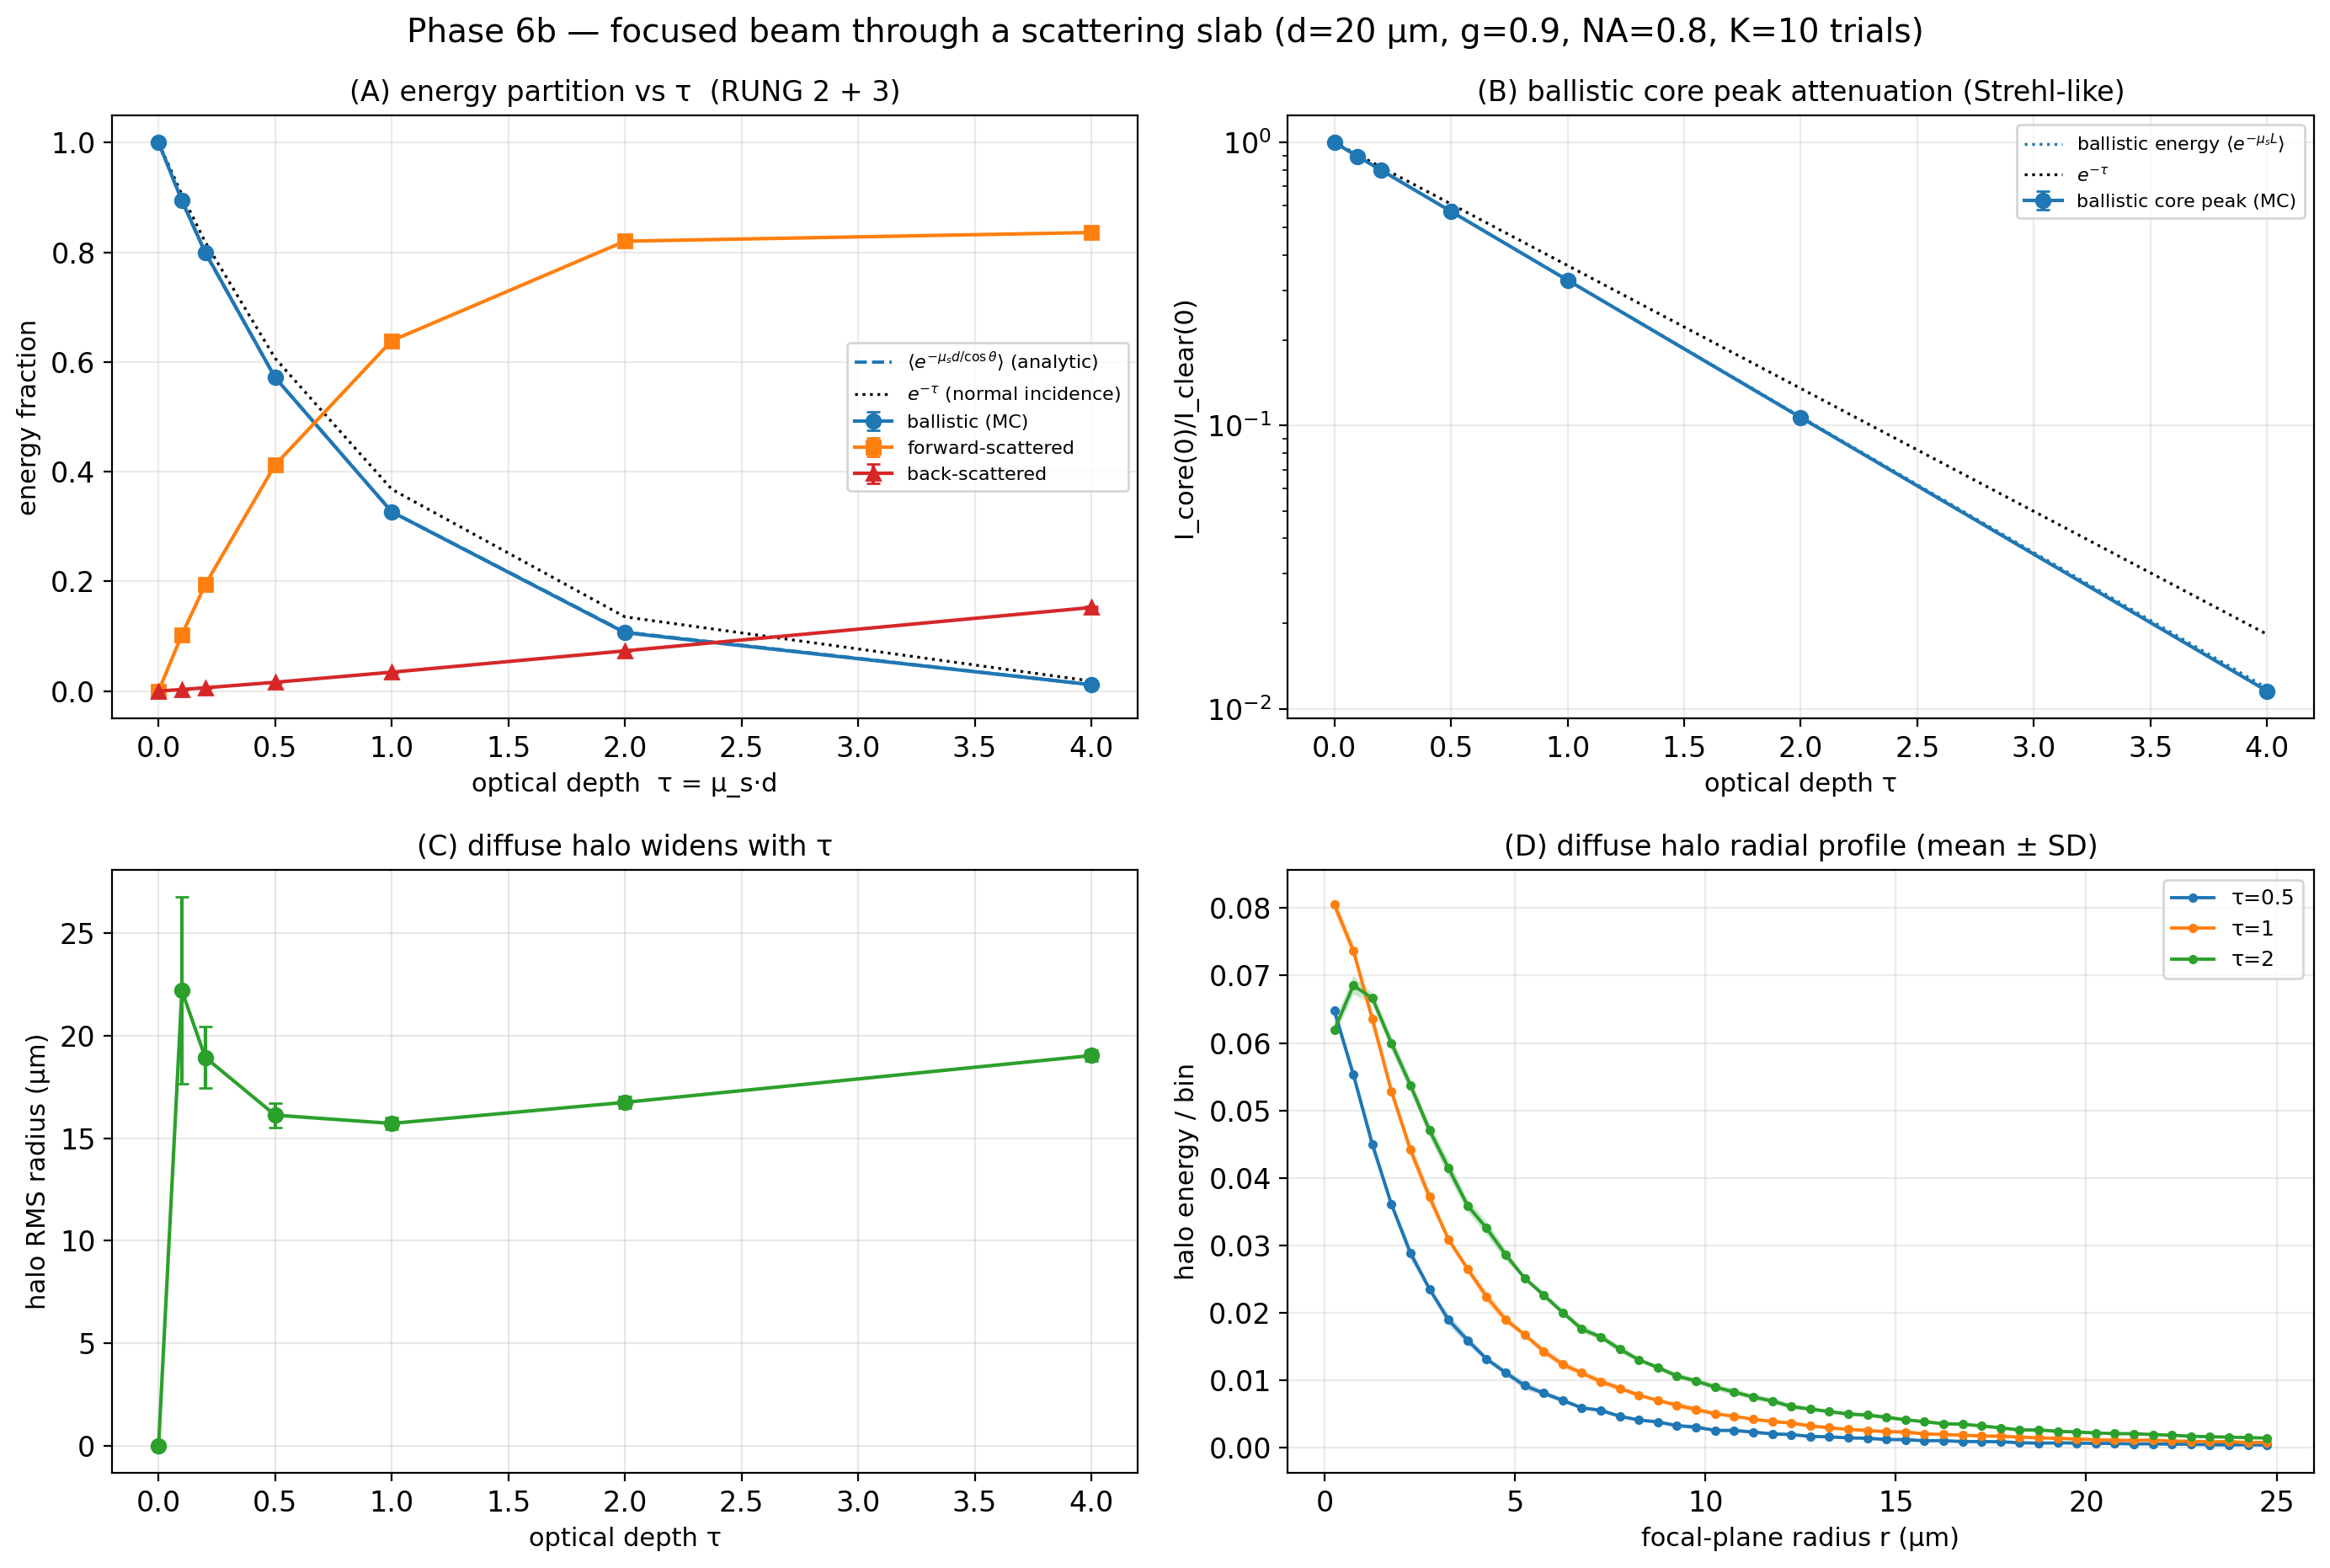
\includegraphics[width=0.99\textwidth]{verify_mc_scatter.png}\end{center}
\textbf{Next:} validation rungs 4--6 (single-scatter Born, diffusion asymptote,
MCML cross-check); the axial halo; and vector $+$ pulsed ($\lambda$-dependent
$\mu_s$) scattering.
\end{document}
